\documentclass[12pt, twoside]{report}
\raggedbottom

\usepackage[utf8]{inputenc}
\usepackage{graphicx}
\usepackage[italian]{babel}
\usepackage{csquotes}
\usepackage{lipsum}
\usepackage{fancyhdr}
\usepackage{pdfpages}
\usepackage{wrapfig}
\usepackage{float}
\usepackage{enumitem}
\usepackage{subcaption}
\usepackage{framed}
\usepackage{geometry}
\usepackage{listings,xcolor}
\usepackage{inconsolata}
\usepackage{setspace}
\usepackage[T1]{fontenc}
\usepackage[backend=biber, sorting=none]{biblatex}
\usepackage{hyperref}
%\usepackage[nottoc,numbib]{tocbibind}

\hypersetup{
  colorlinks=false,
  hidelinks,
  pdftitle={Integrazione Interfaccia e Elaborazione Dati per il Progetto PRISMA}
}
\DeclareCaptionFormat{custom}
{%
    \textbf{#1#2}#3
}
\captionsetup{format=custom}

\renewenvironment{shaded}{%
  \def\FrameCommand{\fboxsep=\FrameSep \colorbox{shadecolor}}%
  \MakeFramed{\advance\hsize-\width \FrameRestore\FrameRestore}}%
 {\endMakeFramed}
 \definecolor{shadecolor}{gray}{0.9}

%\graphicspath{ {images/} }
\addbibresource{impaginazione/references.bib}

\fancypagestyle{plain}{%
  \fancyhf{}
  \fancyfoot[LE,RO]{\thepage}
  \renewcommand{\headrulewidth}{0pt}}
\renewcommand{\chaptermark}[1]{\markboth{#1}{}}
\renewcommand{\sectionmark}[1]{\markright{#1}}

\pagestyle{fancy}

\fancyhead[LO]{\scshape\nouppercase{\rightmark}}
\fancyhead[RE]{\scshape\nouppercase{\leftmark}}
\fancyhead[LO,RE]{\itshape\nouppercase{\rightmark}}
\fancyhead[LE,RO]{\textsc{\leftmark}}

\fancyfoot[LE, RO]{\scshape \thepage}
\fancyfoot[CO,CE]{}

\definecolor{dkblue}{rgb}{0,0,.6}

\lstdefinelanguage{JavaScript}{
  keywords={typeof, new, true, false, catch, function, return, null, catch, switch, var, if, in, while, do, else, case, break},
  ndkeywords={class, export, boolean, throw, implements, import, this},
  sensitive=false,
  comment=[l]{//},
  morecomment=[s]{/*}{*/},
  morestring=[b]',
  morestring=[b]"
}

\lstdefinestyle{PHP}{
  language        = php,
  basicstyle      = \small\ttfamily,
  keywordstyle    = \color{dkblue},
%  stringstyle     = \color{purple},
  commentstyle    = \color{gray},
  showstringspaces= false
  frame           = top,
  frame           = bottom,
  aboveskip       = 1.5em,
  belowskip       = 1.5em,
  emph            =[1]{php},
  emphstyle       =[1]\color{black},
  emph            =[2]{if,and,or,else, return, public, static, function},
  emphstyle       =[2]\color{cyan}}
  
\lstdefinestyle{JavaScript}{
  language        = JavaScript,
  basicstyle      = \small\ttfamily,
  keywordstyle    = \color{dkblue},
%  stringstyle     = \color{purple},
  commentstyle    = \color{gray},
  showstringspaces= false
  frame           = top,
  frame           = bottom,
  aboveskip       = 1.5em,
  belowskip       = 1.5em,
  emph            =[1]{php},
  emphstyle       =[1]\color{black},
  emph            =[2]{if,and,or,else, return, public, static, function},
  emphstyle       =[2]\color{cyan}}

\begin{document}

%\begin{titlepage}
%  
\includepdf{frontespizio}
%\end{titlepage}

\newgeometry{margin=1in}
\begin{titlepage}
        
        \noindent
        \begin{minipage}[t]{0.19\textwidth}
            \vspace{-4mm}{
\includegraphics[scale=1.15]{impaginazione/logo_unimib.pdf}}
        \end{minipage}
        \begin{minipage}[t]{0.81\textwidth}
        {
                \setstretch{1.42}
                {\textsc{Università degli Studi di Milano - Bicocca}} \\
                \textbf{Scuola di Scienze} \\
                \textbf{Dipartimento di Informatica, Sistemistica e Comunicazione} \\
                \textbf{Corso di laurea in Informatica} \\
                \par
        }
        \end{minipage}
        
	\vspace{40mm}
        
	\begin{center}
            {\LARGE{
                    \setstretch{1.2}
                    \textbf{Integrazione Interfaccia e Elaborazione \\ Dati per il Progetto PRISMA}
                    \par
            }}
        \end{center}
        
        \vspace{40mm}

        \noindent
        {\large \textbf{Relatore:} Prof. Giuseppe Vizzari} \\

        \noindent
        {\large \textbf{Correlatore:} Ing. Andrea Novati}
        
        \vspace{15mm}

        \begin{flushright}
            {\large \textbf{Relazione della prova finale di:}} \\
            \large{Elisa Pioldi} \\
            \large{Matricola 856591} 
        \end{flushright}
        
        \vspace{30mm}
        \begin{center}
            {\large{\bf Anno Accademico 2021-2022}}
        \end{center}

        \restoregeometry
        
\end{titlepage}
\restoregeometry
\newgeometry{width=150mm,top=25mm,bottom=25mm,headheight=15pt}

\newpage
\thispagestyle{empty}
\begin{flushright}
\null\vspace{\stretch{1}}
\textit{A tutti quelli che hanno creduto in me anche quando io non l'ho fatto.}
\vspace{\stretch{2}}\null
\end{flushright}

\tableofcontents

\chapter{Introduzione - Progetto PRISMA}
\begin{center}
\emph{PRISMA (Prima Rete Italiana per la Sorveglianza sistematica di Meteore e
Atmosfera)\footnote{Da qui in avanti ci si riferirà ad essa solo con la sigla corrispondente.} è un progetto collaborativo proposto e coordinato dall’Istituto Nazionale
di Astrofisica (INAF) a cui partecipano Istituti di ricerca, associazioni, scuole.
L’elenco completo dei partecipanti è disponibile sul sito www.prisma.inaf.it}
\end{center}

\section{Il Progetto}
\begin{wrapfigure}{l}{0.3\textwidth}
    \vspace{-30pt}
    \begin{center}
    
\includegraphics[width=0.3\textwidth]{images/logo.png}
    \end{center}
    \vspace{-22pt}
\end{wrapfigure}

Il progetto PRISMA prevede la realizzazione di una rete italiana di camere all-sky per l'osservazione di meteore brillanti (fireball e bolidi), al fine di determinare le orbite degli oggetti che le provocano e delimitare con un buon grado di approssimazione le aree dell'eventuale caduta di frammenti per poter recuperare le meteoriti.

Il monitoraggio sistematico della copertura nuvolosa e dell'attività elettrica sarà usato per la validazione di modelli meteorologici. I dati raccolti in maniera sistematica contribuiranno al perfezionamento dei modelli di interazione dei corpi cosmici con l'atmosfera che a tutt'oggi presentano ancora molte lacune a causa della mancanza di dati osservativi di qualità.
\cite{progetto-PRISMA}


\section{Fireball e Bolide}
Fireball e bolide sono termini astronomici per indicare meteore particolarmente brillanti e spettacolari che possono essere agevolmente viste anche di giorno da un'ampia regione. 

Per meteoroide si intende un frammento di asteroide o cometa in orbita attorno al Sole che ha una dimensione inferiore al metro. Le meteore, anche chiamate stelle cadenti, sono la traccia visibile dei meteoroidi che entrano nell'atmosfera terrestre con un'alta velocità. 

Un fireball è una meteora che raggiunge una luminosità uguale o superiore a quella di Venere, il terzo astro più brillante nel cielo. I fireball che esplodono e si frammentano durante la caduta sono chiamati in gergo tecnico bolidi, anche se i due termini sono spesso utilizzati indifferentemente. Durante la fase di ingresso in atmosfera, l'oggetto impattante è rallentato e riscaldato per attrito. Nella parte frontale il gas atmosferico è compresso e scaldato e forma una zona di shock. Parte dell'energia generata dall'attrito provoca l'erosione dell'oggetto, e nella maggior parte dei casi la sua successiva rottura. La frammentazione aumenta l'effetto dell'attrito, causando ulteriore erosione e frammentazione, fino a quando la differenza tra le forze di pressione di fronte e dietro l'oggetto ne provocano la completa e catastrofica distruzione. Sebbene in genere gli oggetti che generano un fireball non siano grandi a sufficienza per sopravvivere intatti al passaggio in atmosfera, spesso frammenti o meteoriti possono venir recuperati a terra.
\cite{bolide-fireball}

\section{Enti Coinvolti}
Al progetto partecipano ricercatori dell'Istituto Nazionale di Astrofisica e delle Università, Gruppi Astrofili e Osservatori Astronomici e Meteorologici regionali e locali. Anche le Scuole sono coinvolte con un programma didattico e con laboratori di astronomia che intendono far partecipare gli studenti e i singoli cittadini alle attività di ricerca del progetto, fianco a fianco con i ricercatori. Questo aspetto del progetto si situa nell'ambito di PRISMA-Edu, che viene sviluppato grazie anche al sostegno finanziario delle fondazioni bancarie. \cite{progetto-PRISMA}

Per quanto riguarda il lato informatico del progetto, PRISMA si appoggia all'azienda esterna N3 Srl \cite{n3srl}. Il progetto illustrato nei successivi capitoli è avvenuto in collaborazione con questa azienda.

\begin{figure}[b]

\begin{subfigure}{\textwidth}
\begin{center}
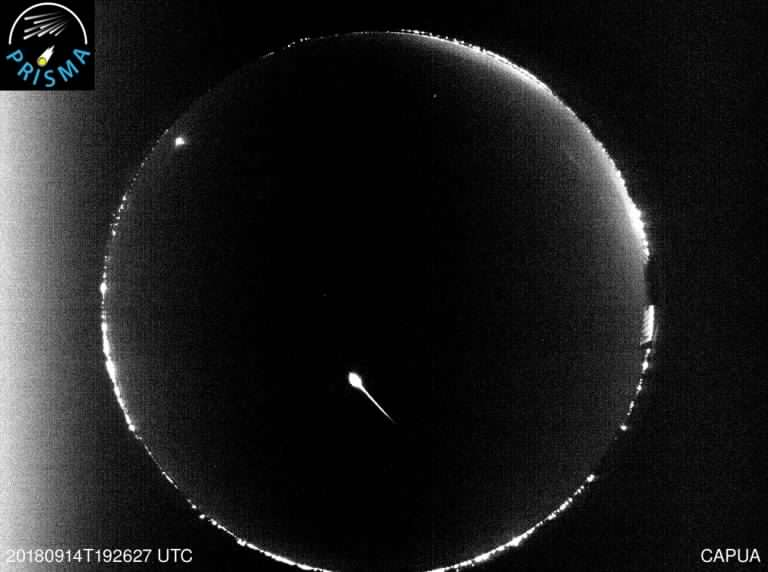
\includegraphics[width=0.9\textwidth]{images/CAPUA_20180914.jpg}
\caption{Rilevazione del 14/09/18 19:26:08 UTC}
\end{center}
\end{subfigure}

\vspace{12pt}

\begin{subfigure}{\textwidth}
\begin{center}
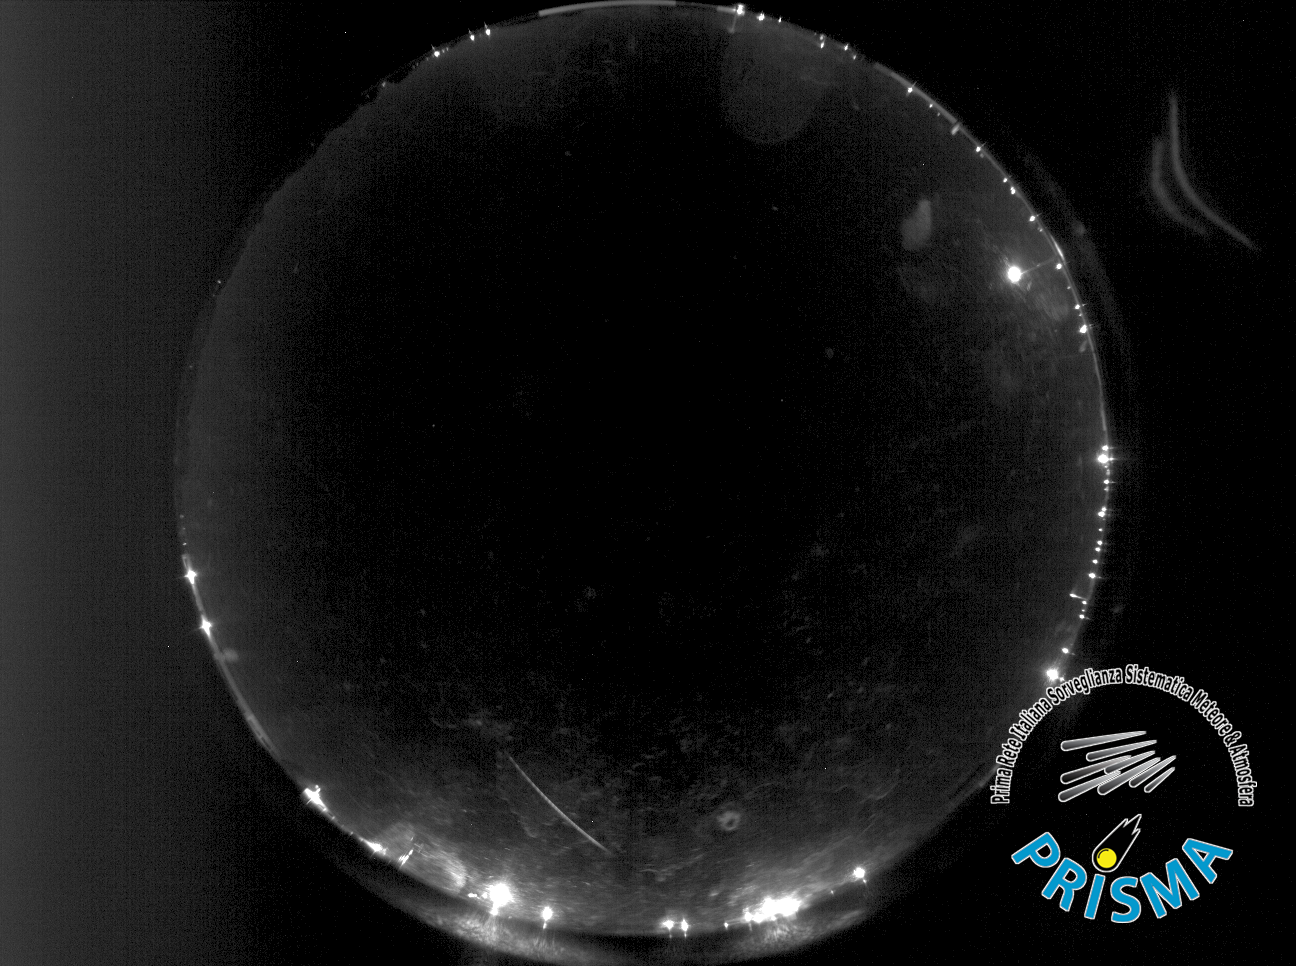
\includegraphics[width=0.9\textwidth]{images/CODOGNO_22062022.png}
\caption{Rilevazione del 22/06/22 00:12:00 UTC}
\label{fig:codogno-2206}
\end{center}
\end{subfigure}

\caption{Rilevazioni di meteore ad opera di PRISMA}
\end{figure}

\chapter{Requisiti dell'Attività}
\section{Interazione Utente - Nodo}
La rete si compone di diversi nodi, chiamati \textbf{stazioni}, distribuiti in tutta Italia, ciascuno dei quali è associato ad una \textbf{telecamera} che rileva gli eventi atmosferici.

Si illustra di seguito come prende luogo l'interazione tra l'utente e il nodo, con lo scopo di contestualizzare il lavoro svolto.

\subsection{Struttura e accesso al nodo}
Sui nodi sono in esecuzione il software FreeTure (cfr. sezione \ref{freeture}) e Prometheus (cfr. sezione \ref{prometheus}) con relative configurazioni; inoltre le funzioni del nodo sono organizzate e gestite tramite diversi container (cfr. sezione \ref{docker}).
L'utente può accedere al nodo tramite un'apposita \textbf{VPN} (cfr. sezione \ref{rete-VPN}) in SSH.

\subsection{Dati raccolti} \label{dati-raccolti}
La telecamera del nodo riprende i fenomeni atmosferici e grazie a FreeTure produce tre tipi di dati, memorizzati nel file system del nodo e consultabili dall'utente connettendosi in SSH:
\begin{enumerate}
    \item \textbf{Capture} (o \textbf{calibrazioni}): immagini di “calibrazione”, sono scattate ogni 10 minuti. Vengono utilizzate per mappare la porzione di cielo corrispondente e calibrare gli strumenti necessari.
    \item \textbf{Stack}: immagini che forniscono una sorta di “cronologia”, vengono scattate ogni minuto.
    \item \textbf{Detection}: vengono generate al verificarsi di un evento atmosferico. A differenza delle \emph{capture} e degli \emph{stack} non sono costituite da un'unica immagine ma da un insieme di file, tra cui i frame che individuano l'evento.
\end{enumerate}
Tutte le immagini prodotte sono nel formato FITS, formato standard della NASA usato in astronomia \cite{FITS}. 

Il progetto prima dell'inizio del tirocinio constava già di un'ampia infrastruttura tra cui si annovera una serie di procedure sul server di elaborazione centrale per la generazione di eventi e un sistema di automazione embrionale per gli script sul server.

Gli eventi singoli (\emph{detection}) provenienti dai nodi vengono infatti sincronizzati giornalmente sul server di elaborazione da una procedura dedicata. Devono essere elaborati dal nodo di elaborazione centrale per poter generare gli eventi multipli, che vengono generalmente definiti come eventi ripresi da almeno tre nodi della rete. Solo a questo punto un evento multiplo può denotare un fenomeno atmosferico importante, come l'effettivo passaggio di una meteora.

\section{Implementazione}
Si è reso necessario fornire un'interfaccia accessibile tramite web browser per la modifica delle configurazioni e la gestione dei software operanti sui singoli nodi, nonché per rendere più veloce e pratica la consultazione dei dati raccolti. Si è voluto quindi elaborare le immagini e i file per permettere all'utente di interpretare in modo immediato e con facilità i dati raccolti dal nodo.

Queste richieste si sono tradotte con l'implementazione di una web application accessibile tramite VPN (cfr. sezione \ref{rete-VPN}) utilizzando come URL l'indirizzo IP del nodo. L'oggetto del tirocinio è stato quindi lo sviluppo di questa web app sia backend sia frontend.

\chapter{Tecnologie Abilitanti}
\section{Linguaggi, Librerie, Software} \label{software}
Per realizzare la web application sono stati utilizzati diversi linguaggi di programmazione, framework e software. Per comodità si distinguono quelli utilizzati lato client e lato server. 

\subsection{Lato client}

Per l'implementazione e la progettazione dell'interfaccia grafica sono stati adoperati:

\begin{itemize}
    
\item
\textbf{JavaScript} \cite{JS}: linguaggio di programmazione di alto livello. Permette la tipizzazione dinamica ed è multi-paradigma: è orientato agli eventi, funzionale e supporta la programmazione di tipo imperativo. È utilizzato principalmente nella programmazione Web lato client.
    
\item
\textbf{jQuery} \cite{jQuery}: libreria JavaScript piccola, veloce e ricca di funzionalità. Rende la manipolazione HMTL, la gestione di eventi, le animazioni e Ajax molto più semplici con una API semplice da utilizzare che funziona attraverso un grande varietà di browser.
    
\item
\textbf{Google Maps} \cite{GoogleMaps}: API di JavaScript fornita da Google. Permette di personalizzare mappe mostrate su pagine web e dispositivi mobili. Maps per Javascript mette a disposizione quattro tipi base di mappa che possono essere modificati utilizzando livelli e stili, controlli ed eventi, e vari servizi e librerie.
    
\item
\textbf{HTML}: letteralmente \emph{HyperText Markup Language}, è un linguaggio di markup gerarchico strutturato ad albero. Permette di formattare e impaginare pagine Web.
    
\item
\textbf{CSS}: \emph{Cascading Style Sheets} testualmente, descrive come gli elementi HTML devono essere visualizzati e permette di formattare lo stile delle pagine.

\item
\textbf{Bootstrap} \cite{Bootstrap}: kit di strumenti per il front-end. Consente di costruire e personalizzare con Sass e utilizzare sistemi a griglia e componenti precostituiti.
In particolar modo la web application si serve del \emph{Grid System} di Bootstrap per adattarsi dinamicamente al dispositivo.

\end{itemize}

\subsubsection{DataTables} \label{datatables}

Data la complessità di questo plug-in è necessario dedicare una spiegazione più approfondita al loro impiego specifico in questo progetto, per evidenziare le funzionalità che sono state utilizzate.

\textbf{DataTables} \cite{DataTables} è un plug-in per la libreria jQuery di JavaScript. È uno strumento molto flessibile, costruito sulle fondamenta del miglioramento progressivo, che aggiunge delle funzionalità avanzate ad ogni tabella HTML.
Nel progetto viene ampiamente sfruttata la funzionalità server-side processing, per la gestione di grandi quantità di dati lato server.

Inizializzando una DataTable si definiscono tutta una serie di parametri e valori, in questo caso i parametri più utilizzati o di maggior importanza sono stati:
\begin{itemize}
    \item \texttt{oLanguage}: dà la possibilità di rinominare come si preferisce le \emph{label} di una DataTable;
    \item \texttt{columnDefs}: permette di definire specifiche sulle colonne della tabella, ad esempio formattando il testo in esse presente, aggiungere elementi HTML o nascondere le colonne in questione;
    \item \texttt{fnServerParams}: si inseriscono ulteriori parametri da inviare al server quando richiede i dati; il progetto ne ha usufruito per specificare al server di quale giorno mandare i dati;
    \item \texttt{rowGroup}: raggruppa i dati come specificato; nell'app è stato impiegato per raggruppare i dati per giorni;
    \item \texttt{drawCallback}: specifica una funzione da chiamare ogni volta che la tabella viene aggiornata.
\end{itemize}

\begin{lstlisting}[style=JavaScript,caption={Parte dell'implementazione della DataTable della sezione \ref{ft-conf-automatica}},captionpos=b,label={lst:esempio-datatable}]
table = $('#FreetureFinalList').DataTable({
        "oLanguage": {
            "sZeroRecords": "Nessun risultato",
            "sSearch": "Cerca:",
            "oPaginate": {
                "sPrevious": "Indietro",
                "sNext": "Avanti"
            },
            "sInfo": "Mostra pagina _PAGE_ di _PAGES_",
            "sInfoFiltered": "",
            "sInfoEmpty": "Mostra pagina 0 di 0 elementi",
            "sEmptyTable": "Nessun risultato",
            "sLengthMenu": "Mostra _MENU_ elementi"
        },
        "columnDefs": [
            {
                "targets": [-1, -2, -3],
                "visible": false
            }],
        responsive: true,
        "fnServerParams": function (aoData) {
            // Show page with passed index
            aoData.push({"name": "searchPageById", "value": 
                indexToShow});
        },
        [...]
        "iDisplayLength": 10,
        "iDisplayStart": 0,
        "pageLength": 10,
        bProcessing: true,
        bServerSide: true,
        bStateSave: true,
        sAjaxSource: '/lib/ft/V2/freeturefinal/datatable/list',
        "paging": true,
        "ordering": false,
        "info": true,
        "searching": false
    });
\end{lstlisting}

Una funzionalità supportata da DataTables è il \emph{server-side processing} con paginazione lato client: in questo modo vengono richiesti solo i dati mostrati nella pagina corrente allo specifico endpoint (\texttt{sAjaxSource}) e non si deve appesantire il client con lo scaricamento di una consistente mole di dati. Questa caratteristica è risultata ad esempio molto utile nelle sezioni \ref{sezione-capture-stack} e \ref{sezione-detection}, dove i dati da processare sono numerosi e consistenti.

I dati ricevuti dal server (strutturati in un oggetto specifico che il client può interpretare) vengono poi mostrati secondo le indicazioni nella tabella.

\begin{lstlisting}[style=PHP,caption={Esempio di oggetto inviato al client per estrarre i dati da inserire nella DataTable. I dati veri e propri sono in \texttt{aaData}.},captionpos=b]
[...]
$output = array(
        "sEcho" => intval($_GET['sEcho']),
        "pageToShow" => $pageNumber,
        "iTotalRecords" => $iTotal,
        "iTotalDisplayRecords" => $iTotal,
        "aaData" => $reply
    );
return $output;
\end{lstlisting}

In alcune sezioni si è avuto il bisogno di inserire in alcune colonne non solo un dato testuale, ma un vero e proprio elemento HTML, sia che fosse un testo formattato o addirittura un pulsante. In questo caso si è usufruito del parametro \texttt{columnDefs} e la funzione \texttt{render}. Di seguito si trova il codice implementato per realizzare un pulsante di download:

\begin{lstlisting}[style=JavaScript,caption={Realizzazione del pulsante di download nella DataTable della sezione \ref{sezione-capture-stack}.},captionpos=b]
[...]
{
    "targets": [-1],
    render: function (data, type, row, meta) {
        return "<center>" + 
               "<a href='/lib/capture/V2/capture/download/" + 
               data + "'>" + 
               "<button class='btn btn-success'> +
               "<i class='fa fa-download'>" +
               "</i></button>" +
               "</a></center>";
    }
}
[...]
\end{lstlisting}

\subsection{Lato server}

Per realizzare il lato server della web application sono stati utilizzati i seguenti linguaggi e framework:

\begin{itemize}

    \item \textbf{PHP} \cite{PHP}: linguaggio di scripting \emph{general-purpose} adatto soprattutto allo sviluppo web. 
    
    \item \textbf{Symfony} \cite{Symfony}: insieme di componenti PHP riutilizzabili e framework PHP per progetti web. Nella sezione \ref{framework-N3} si illustra nel dettaglio quali componenti si sono utilizzati.
    
    \item \textbf{Silex} \cite{Silex}: micro-framework PHP per sviluppare siti web basati su componenti Symfony.
    
\end{itemize}

\noindent Relativamente all'elaborazione dei dati sono stati impiegati i software elencati di seguito, che permettono l'interazione da linea di comando: 

\begin{itemize}

    \item \textbf{fitspng} \cite{fitspng}: convertitore di immagini dal formato astronomico FITS in formato PNG. Risulta essere fondamentale per la visualizzazione da parte dell'utente delle immagini rilevate dalla telecamera in un formato che il browser può renderizzare.
    
    \item \textbf{ImageMagick} \cite{ImageMagick}: permette di creare, modificare, comporre o convertire immagini digitali. È stato impiegato per applicare un watermark alle immagini visualizzate dall'utente.
    
    \item \textbf{FFmpeg} \cite{FFmpeg}: soluzione \emph{cross-platform} completa per registrare, convertire e eseguire lo streaming di audio e video. Nel dettaglio, per l'implementazione della web application è stata utilizzata per comporre un video da un insieme di fotogrammi e per applicare un watermark al video generato.
    
    \item \textbf{libzip} \cite{libzip}: libreria in C per leggere, creare e modificare archivi zip. Il suo utilizzo ha avuto luogo per fornire all'utente un archivio dell'insieme di file che compongono una detection (cfr. sezione \ref{dati-raccolti}).
    
    \item \textbf{sysstat} \cite{sysstat}: pacchetto software che contiene diverse funzionalità, comuni a molti sistemi Unix, per monitorare le performance del sistema e l'attività di utilizzo. È risultato fondamentale per ricavare l'utilizzo della CPU (cfr. sezione \ref{stato-risorse-hw}).

\end{itemize}

Per utilizzare i software citati, viene adoperato il metodo PHP \texttt{shell\_exec()} nel codice eseguito sul server, che consente di eseguire il comando tramite shell e restituire l'output completo come stringa.

\section{Infrastruttura PRISMA} \label{infrastruttura-PRISMA}
Il progetto PRISMA si articola in una complessa struttura che si sviluppa tra diverse componenti software e architetturali. Nelle sottosezioni a seguire verranno illustrati quelle principali con cui si è interagito o che si sono adoperate lungo lo svolgimento del progetto.

\subsection{Framework N3} \label{framework-N3}

\begin{wrapfigure}{r}{0.3\textwidth}
    \vspace{-34pt}
    \begin{center}
    
\includegraphics[width=0.3\textwidth]{images/logo_orma.png}
    \end{center}
    \vspace{-30pt}
\end{wrapfigure}
Nella sezione \ref{software} si è accennato all'uso di PHP e JavaScript con alcuni relativi framework. Tra di essi si annovera il framework sviluppato dall'azienda N3 con cui è avvenuta la collaborazione del progetto: \textbf{Orma - \emph{Management System}}.
Il framework si avvale di PHP (e Symfony), JavaScript e DataTables, è modellato su un \textbf{pattern MVC} ed è orientato all'interazione con gli oggetti, che possono essere visualizzati, aggiunti, modificati o cancellati, mediante una visualizzazione tabellare. 
Originariamente si basava sull'interazione con un database, ma in questo caso è stato adattato per lavorare con i dati presenti sul \textbf{file system} del nodo; inoltre nonostante si sia preservata la struttura base è stato necessario, data la complessità del progetto, svincolare da alcuni paradigmi lungo lo sviluppo del sito. La struttura del framework è molto complessa, si presentano qui dunque i dettagli più importanti per comprenderne il funzionamento generale.

Il framework è stato progettato per gestire un insieme di \textbf{oggetti} con cui l'utente può interagire.
Impone quindi la realizzazione di una web application divisa in diverse \textbf{sezioni}, ciascuna delle quali è inerente ad una classe di oggetti presente sul database (o file system). Su ogni oggetto possono essere effettuate varie \textbf{operazioni}:
\begin{itemize}[noitemsep,nolistsep]
    \item \textbf{Visualizzazione} (\emph{get})
    \item \textbf{Inserimento} (\emph{insert})
    \item \textbf{Modifica} (\emph{edit})
    \item \textbf{Cancellazione} (\emph{delete})
\end{itemize}

\subsubsection{Lato client}

Ad ogni operazione su ciascuna classe di oggetti è associata una pagina HTML diversa, a cui si ha accesso tramite una gestione a \textbf{controller}, secondo il paradigma di Symfony. Accedendo a ciascuna sezione secondo i collegamenti predisposti graficamente, i controller reindirizzano l'utente a URL specifici a seconda dell'operazione che è richiesta eseguire sull'oggetto, occupandosi di gestire anche una prima parte di sicurezza degli accessi. 

Nella seguente spiegazione del flusso dell'applicazione ci si sofferma soprattutto sull'operazione di \textbf{modifica}, siccome è l'unica utilizzata nell'applicazione illustrata.

Per ogni sezione è presente una pagina di script JS (chiamata come la classe dell'oggetto, le classi degli oggetti si chiamano invece con il nome della classe e il suffisso \texttt{Class}), che gestisce gli eventi diretti generati dalle interazioni dell'utente con il sito e le operazioni principali con appositi metodi (ad esempio, \texttt{editObj()} per la modifica). Ciascuna sezione mostra una \textbf{tabella}, realizzata con DataTables, che elenca gli oggetti della classe con i rispettivi attributi presenti del database. Ad esempio, la sezione \emph{Utenti} avrà una tabella con una riga per ogni utente presente nel DB e due colonne che corrisponderanno a username e livello, ovvero gli attributi dell'utente. Inoltre sotto la tabella è presente un \emph{form} con tanti campi quanti sono gli attributi dell'oggetto: cliccando sulla riga corrispondente, il sistema riempie automaticamente i campi con gli attributi esistenti e l'utente ha la possibilità di modificarli e inviare le modifiche. 

Le operazioni sugli oggetti prima di essere inviate come richieste al server passano attraverso una complessa pipeline.
Si deve dunque implementare per ciascuna classe di oggetti una classe che mandi le informazioni da elaborare allo script \texttt{form.js} (che si chiamerà con il nome della classe con il suffisso \texttt{Logic}) e una classe che riceve i dati elaborati da quest'ultimo e interagisca con il server (che avrà il nome della classe con l'aggiunta del suffisso \texttt{Factory}). Le classi \texttt{-Logic} sono particolari perché contengono un unico dizionario le cui chiavi sono le classi e i valori le funzioni chiamate nello script \texttt{form.js}.

Lo script \texttt{form.js} ha il compito di gestire il riempimento dei campi nel form di modifica, la validazione dei campi attraverso un apposito sistema di validazione, la distinzione delle operazioni (ad esempio se l'utente ha richiesto la modifica di un oggetto esistente oppure l'aggiunta di uno nuovo), la visualizzazione di messaggi di successo o di errore, l'aggiornamento delle tabelle e così via.

Le classi \texttt{-Factory} interagiscono infine con un'ultima classe che contiene dei metodi appositi per eseguire le chiamate AJAX al server.

\subsubsection{Lato server}

Per quanto riguarda il server, la logica è divisa anche in questo caso ad oggetti. Ciascun oggetto è gestito da un insieme di classi PHP che ricevono le richieste e operano sul database.

In particolar modo, gli endpoint delle richieste sono gestiti con il micro-framework Silex. Ogni endpoint è relativo ad una singola operazione o alla generazione di una tabella. Similmente al lato client, dal file \emph{index} l'operazione da eseguire attraversa una pipeline composta da diverse classi fino alla creazione di una query da effettuare sul database. Siccome il progetto non si affidava ad un database, si tralascia la spiegazione dettagliata della pipeline, la maggior parte del lavoro si è focalizzato su un'unica classe in cui implementare i metodi necessari.

\subsubsection{Modifiche al framework}

Dal momento che il progetto PRISMA è più complesso e non necessita di una semplice gestione di oggetti su database, sono state apportate delle modifiche e delle integrazioni:
\begin{itemize}
    \item Si è introdotto il caricamento/scaricamento di file e immagini indipendenti dai singoli oggetti;
    \item Si sono implementate delle sezioni non inerenti a classi di oggetti, ad esempio la sezione relativa alla VPN (cfr. sezione \ref{sezione-OVPN});
    \item Si è resa necessaria l'integrazione per interagire con il file system del nodo dal momento che il framework era stato progettato per lavorare su un database; di conseguenza è stata rimossa la pipeline per la formulazione di query e si sono implementati metodi per leggere e scrivere direttamente sul file system.
\end{itemize} 

\subsection{Configurazione della macchina} \label{debian}

Su tutti i nodi è installato come sistema operativo \textbf{Debian Bullseye 11.2}.
Una volta che si è configurato il sistema operativo ci si può collegare alla macchina in SSH per installare tutti i software necessari. Nelle sottosezioni a seguire si approfondiranno le configurazioni principali.

Per quanto riguarda i software di base da installare tra i più importanti si citano Git, OpenVPN, SSH, Docker (secondo il manuale ufficiale \cite{install-Docker-Debian}) e \emph{Prometheus Node Exporter} v1.3.1 (scaricabile dal repository GitHub ufficiale \cite{Prometheus-node-exporter-github} e configurato secondo la guida ufficiale \cite{Prometheus-node-exporter}). Si installano poi i driver della scheda di rete e si effettua la configurazione mDNS per risolvere \texttt{'prismanode.local'} con l'ip del nodo.

Si prosegue quindi importando i file script programmati per bash, finalizzati alla corretta inizializzazione dei container (cfr. sezione \ref{docker}), i sorgenti base dell'applicazione e le chiavi private SSH. A questo punto è possibile accedere tramite browser alla schermata di login dell'applicazione (cfr. sezione \ref{accesso-app}) inserendo l'IP del nodo. Sulla porta 9090 è inoltre possibile accedere all'interfaccia grafica di \emph{Prometheus Node Exporter}. 

Nel corso del tirocinio sono state apportate inoltre delle modifiche alla configurazione iniziale della macchina (cfr. sezione \ref{permessi-macchina}).

\subsection{Rete VPN} \label{rete-VPN}

Il nodo è inserito durante la pre-produzione in una VPN provvisoria, \emph{VPN Guest}, con indirizzo IP provvisorio. Una volta che è stato configurato viene collegato invece alla VPN effettiva, comune a tutti i nodi, con indirizzo IP fisso.
Tutte le configurazioni VPN appena illustrate sono realizzate con \textbf{OpenVPN} \cite{OpenVPN}.

L'utente una volta che si collega in VPN può accedere a tutti i nodi in SSH oppure tramite la web application qui discussa, se ne conosce l'indirizzo IP.

\subsection{FreeTure} \label{freeture}

Per riprendere e individuare gli eventi atmosferici, PRISMA si appoggia a \textbf{FreeTure} \cite{FreeTure}, un software open source di rilevamento di meteore usato per monitorare il cielo con camere all-sky GigE per rilavare e registrare stelle cadenti e fireball.
Il software genera immagini in formato FITS \cite{FITS}, fornisce la possibilità di eseguire acquisizioni a lunga esposizione regolari o programmate ed infine dà la possibilità di accumulare fotogrammi per tenere una sorta di cronologia. 

La telecamera del nodo dipende pertanto dalla configurazione FreeTure (i dati di configurazione sono riportati in un unico file) situata in un apposito container (cfr. sezione \ref{docker}), che definisce, tra i valori più degni di nota, le modalità di acquisizione delle immagini, le interazioni con il file system, la calibrazione della telecamera e l'elaborazione degli scatti per l'individuazione di eventi.

\begin{lstlisting}[style=PHP,caption={Parte della configurazione FreeTure che risiede sul nodo di Codogno.},captionpos=b]
[...]
# Name of the station.
STATION_NAME = CODOGNO	
# Station name.
TELESCOP = ITLO06
# Person in charge.
OBSERVER = Eng. Andrea Novati
# Instrument name.
INSTRUME = FREETURE-CAM
# Camera model name.
CAMERA = BASLER1300gm
# Camera focal.
FOCAL = 1.25
# Camera aperture.
APERTURE = 2.0
# Longitude observatory.
SITELONG = 9.6909138
# Latitude observatory.
SITELAT = 45.1638302
# Elevation observatory.
SITEELEV = 58
[...]
\end{lstlisting}

Inoltre, è possibile definire un file formato BMP che si comporta da “maschera” nell'inquadratura della telecamera: qualsiasi evento che si trovi al di fuori della maschera viene ignorato.

\subsection{Architettura dei container e dei volumi} \label{docker}

Sulla macchina associata alla telecamera è installato \textbf{Docker} \cite{Docker}, che gestisce un insieme di container. Nella figura \ref{fig:containers-arch} sono mostrati i vari container e le interazioni tra di essi. 

L'utente accede al nodo tramite VPN Guest o con VPN di produzione in SSH sulla porta 20, oppure tramite la web application sulla porta 80, realizzata con un web server Apache collocato nel container \emph{prisma-orma}\footnote{L'immagine del container è reperibile su Docker Hub \cite{orma-webmin}}. Da quest'ultimo container, è possibile ugualmente accedere in SSH all'host stesso, da cui si può modificare la configurazione VPN (legata all'host e non ai container). 

A questi container, sono associati dei volumi che mappano delle cartelle sull'host: in \emph{orma-src} sono presenti i sorgenti per la web application, mentre in \emph{orma-keys} è presente la parte relativa agli utenti che possono accedere alla web application.

Inoltre tramite server web si può accedere al volume dove risiede la configurazione FreeTure (\emph{freeture-conf}) e a quello dove sono memorizzati i dati raccolti dalla telecamera (\emph{freeture-data}).
Con questi ultimi due volumi interagisce il container \emph{freeture}, legato alla telecamera.

\begin{figure}
\begin{center}
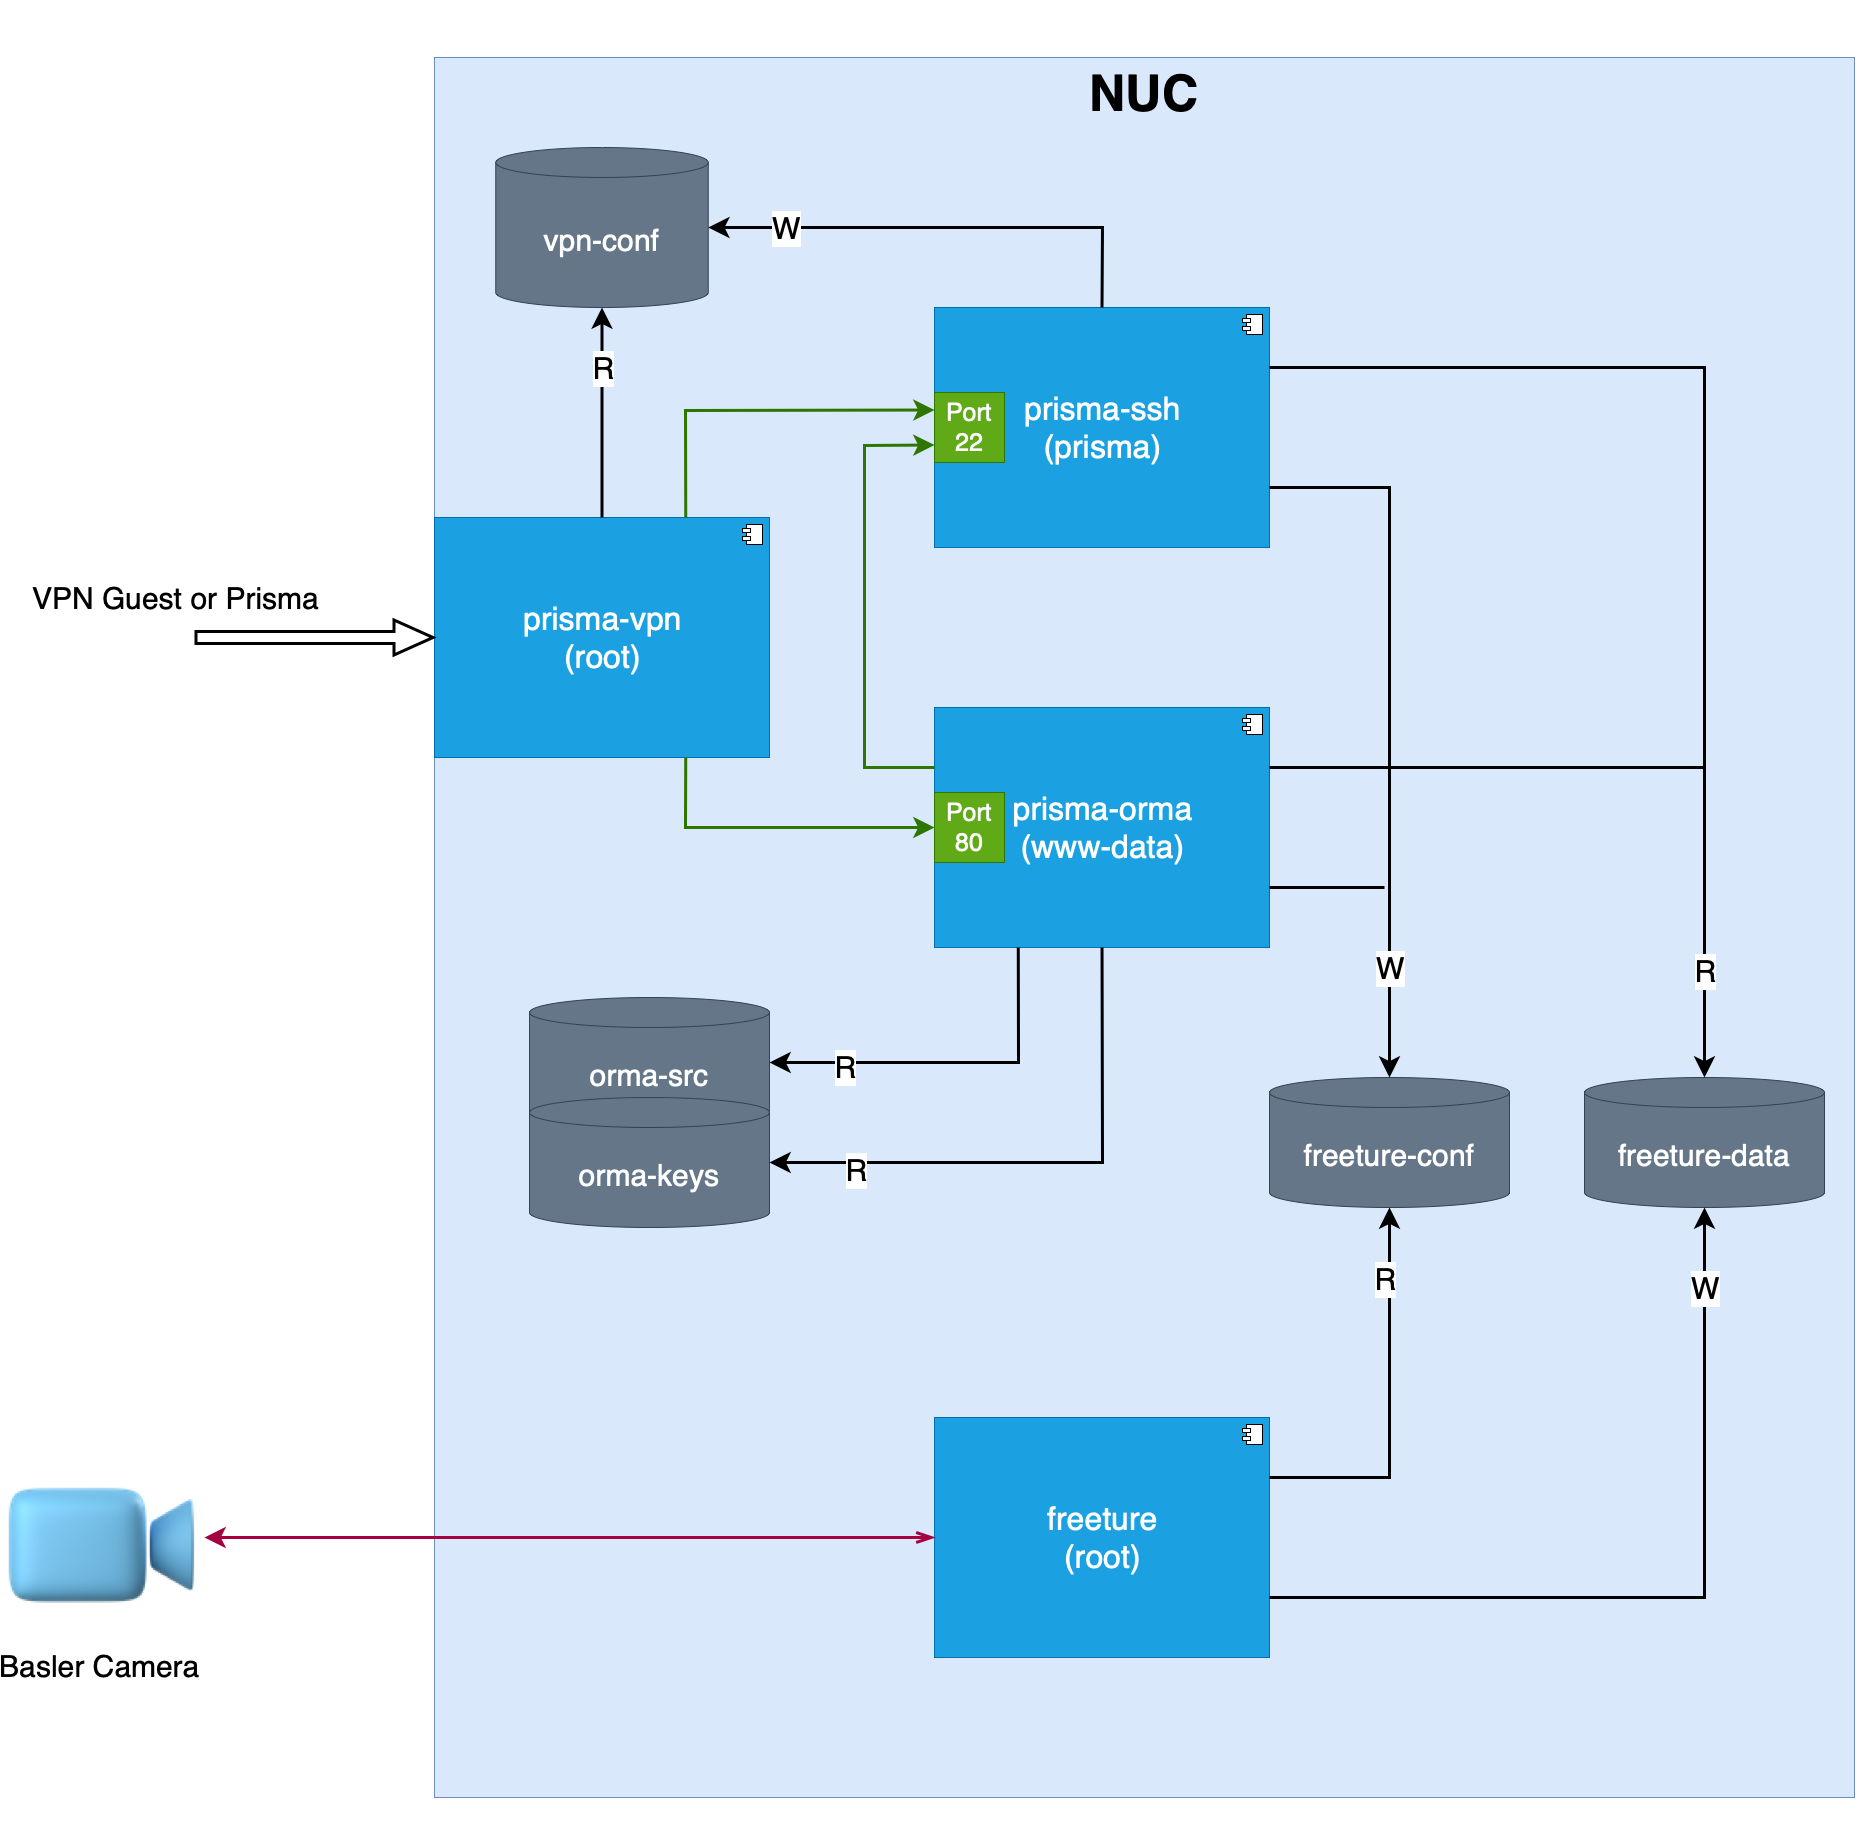
\includegraphics[width=\textwidth]{images/docker-arch.png} 
\caption{Visualizzazione grafica della struttura e delle interazioni dei container.}
\label{fig:containers-arch}
\end{center}
\end{figure}

\subsection{Struttura dati raccolti}

Nella sezione \ref{dati-raccolti} si sono presentati tre tipi di dati: \textbf{capture}, \textbf{stack} e \textbf{detection}. Nel volume \emph{freeture-data} vengono strutturati in una gerarchia ben definita, che verrà riproposta anche nell'interfaccia grafica della web application.

La struttura consta di una cartella per ciascun giorno, all'interno di ciascuna cartella sono presenti ulteriori tre cartelle, una per ogni tipo di dato. Le cartelle relative alle \emph{capture} e agli \emph{stack} sono popolate dai corrispondenti file FITS di quel giorno, mentre quella relativa delle \emph{detection} contiene a sua volta altre cartelle, ognuna coincidente con un evento nel giorno. Tra i file contenuti in quest'ultima cartella ai fini del lavoro svolto si denota la presenza dei fotogrammi, in formato FITS, che catturano la rilevazione, il file FITS principale e i file formato BMP DirMap e GeMap, versioni elaborate della rilevazione che evidenziano la porzione di cielo interessata dall'evento.

\subsection{Prometheus} \label{prometheus}

Le performance del nodo sono controllate tramite il software Prometheus \cite{Prometheus}, un insieme di strumenti per monitorare e notificare sistemi.

In particolar modo sulla macchina è configurato \emph{Prometheus Node Exporter}, che fornisce un'ampia varietà di metriche riguardo all'hardware e al kernel \cite{Prometheus-node-exporter}. Come già accennato, accedendo alla porta 9090 si può accedere all'interfaccia grafica fornita da Prometheus, per avere una panoramica generale delle performance della macchina. Le singole metriche sono invece fruibili sulla porta 9100.

La configurazione di Prometheus risiede sull'host in modo analogo alla VPN.

\begin{figure}[H] 
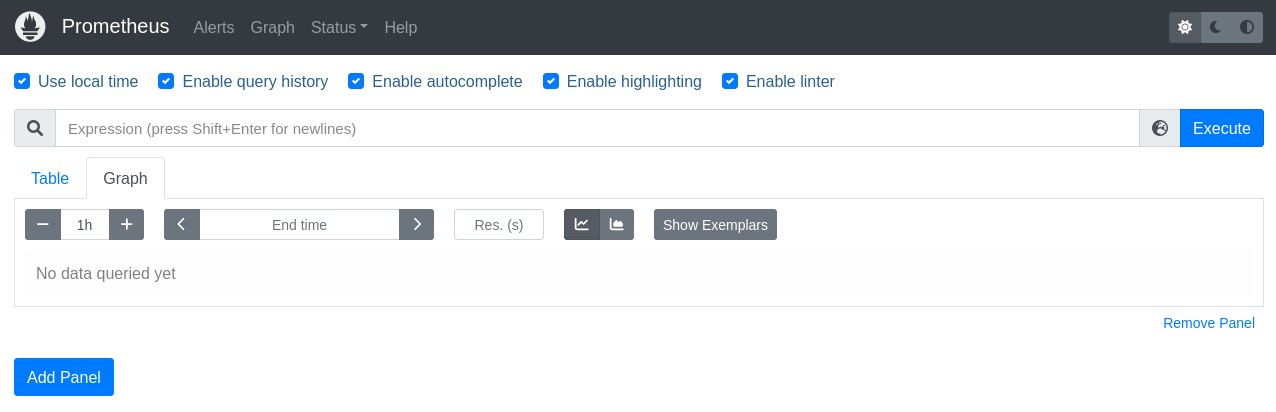
\includegraphics[width=\textwidth]{images/prometheus-9090.jpg} 
\caption{Interfaccia grafica di \emph{Prometheus Node Exporter}.}
\end{figure}

\section{Strumenti di sviluppo} 
Per l'ideazione, lo sviluppo e il testing della web application si è fatto uso dei seguenti strumenti:

\begin{itemize}
    
\item
\textbf{Confluence} \cite{confluence}: workspace per il team dove si possono realizzare pagine dinamiche per creare, catturare e collaborare su qualsiasi idea e progetto.
Il suo impiego è stato destinato alla consultazione e alla stesura della documentazione relativa al progetto PRISMA.

\item
\textbf{NetBeans} \cite{netbeans}: ambiente di sviluppo integrato (IDE) multi-linguaggio. 
È stato utilizzato come IDE per l'implementazione della web application.

\item
\textbf{Oracle VirtualBox} \cite{oracle-vbox}: potente prodotto di virtualizzazione x86 e AMD64 / Intel64.
Con questo strumento si è virtualizzato il nodo di testing illustrato nella sezione \ref{conf-nodo-testing}.

\item
\textbf{Git} \cite{git}: sistema di controllo di versione gratis e open source.

\item
\textbf{GitHub} \cite{github}: servizio di hosting per progetti software. Il lavoro svolto e l'infrastruttura precedentemente realizzata (cfr. sezione \ref{infrastruttura-PRISMA}) è ospitata da questo servizio.

\item
\textbf{Docker Hub} \cite{docker-hub}: servizio di hosting fornito da Docker per trovare e condividere immagini. Le immagini dei container ospitati sul nodo sono qui disponibili.

\item
\textbf{Chrome DevTools} \cite{chrome-devtools}: insieme di strumenti per sviluppatori web integrati direttamente nel browser di Google Chrome. 
Il debug della web application è avvenuto mediante questi strumenti.

\end{itemize}

\chapter{Workflow del Sistema}
In questa sezione, verrà esposto nel dettaglio il lavoro svolto nell'implementazione della web app e delle sue funzionalità durante l'attività di tirocinio, con le eventuali modifiche apportate all'infrastruttura PRISMA (cfr. sezione \ref{infrastruttura-PRISMA}).

\section{Operazioni Preliminari}
\subsection{Configurazione nodo testing} \label{conf-nodo-testing}

Come prima cosa, è stato essenziale configurare una macchina che si comportasse da server per testare le funzionalità della web application.
Inoltre, si è dovuta testare la procedura di configurazione del nodo (cfr. sezione \ref{debian}) per assicurarsi funzionasse pienamente.

A fronte di queste necessità, seguendo il manuale, è stata configurata, utilizzando \textbf{Oracle VM VirtualBox}, una virtual machine \textbf{Debian Bullseye 11.2} ed è stata inserita nella rete VPN Guest (cfr. sezione \ref{rete-VPN}). Tutta l'attività di testing è stata condotta su questa macchina virtuale, collegandosi da client di volta in volta, secondo l'indirizzo IP dinamico corrente.

\subsection{Permessi dei volumi e dei comandi eseguibili} \label{permessi-macchina}

Uno dei primi problemi riscontrati ha riguardato l'accesso da parte di Apache ai volumi dei container. Si è pertanto introdotto uno script che regolasse proprietà e permessi delle cartelle modificabili dalla web app, eseguito ad ogni riavvio della macchina.

Inoltre, il server necessita di eseguire alcuni comandi privilegiati, di conseguenza, in fase di configurazione, all'utente del nodo sono dati i permessi per riavviare il service della VPN e di Prometheus e per eseguire comandi Docker.

\subsection{Integrazione immagine Docker}

Dal momento che il server per elaborare i dati si avvale dei software presentati nella sezione \ref{software}, è stato necessario integrare l'immagine esistente del container \emph{orma-webmin} con l'installazione di:
\begin{itemize}[noitemsep,nolistsep]
    \item fitspng
    \item ImageMagick
    \item FFmpeg
    \item libzip
\end{itemize}

\subsection{Accesso all'applicazione} \label{accesso-app}

Una volta che la macchina viene configurata correttamente e vengono scaricati i sorgenti base da GitHub già esistenti, l'utente può accedere alla schermata di \textbf{login}, dove può inserire nome utente e password (cfr. figura \ref{fig:login}).

\begin{figure}
    \begin{center}
    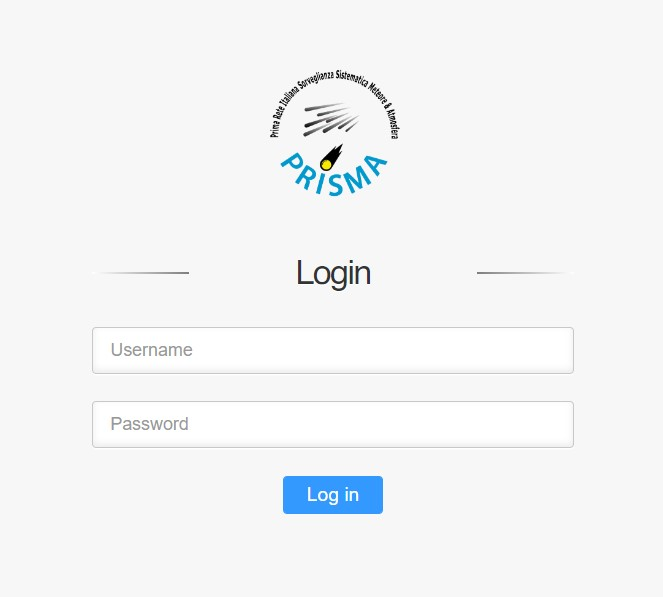
\includegraphics[scale=0.7]{images/login.jpg}
    \caption{Schermata di login.}
    \label{fig:login}
    \end{center}
\end{figure}

Il resto dell'implementazione del sistema è stato oggetto del tirocinio.

\subsection{Menu}

L'utente dopo aver eseguito l'accesso dispone di un menu sulla sinistra per scegliere la sezione di interesse (cfr. figura \ref{fig:menu}). Si noti che alcune funzioni sono nascoste per utenti di livello inferiore (cfr. sezione \ref{sezione-utenti}).

\begin{figure}
    \begin{center}
    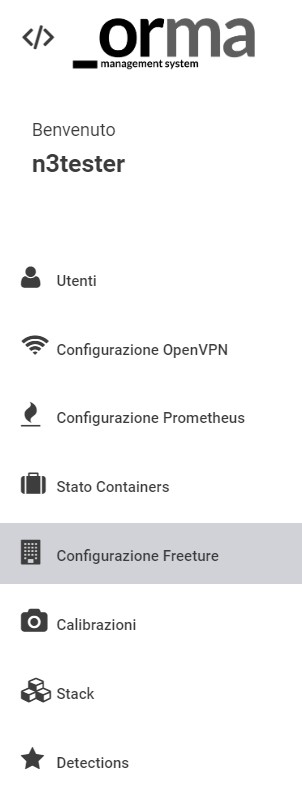
\includegraphics[scale=0.8]{images/menu.jpg}
    \caption{Menu della web application, in questo caso è selezionata la sezione FreeTure.}
    \label{fig:menu}
    \end{center}
\end{figure}

\section{Sezione FreeTure} \label{sezione-freeture}
Selezionando nel menu \emph{Configurazione FreeTure} si accede alla sezione corrispondente dove è possibile modificare la definizione della configurazione del software per il rilevamento di meteore (cfr. figura \ref{fig:freeture}).
Nel dettaglio, si sono dovute realizzare tre sottosezioni differenti:
\begin{enumerate}[noitemsep,nolistsep]
    \item Caricamento di file di configurazione o di maschera
    \item Configurazione automatica
    \item Configurazione manuale
\end{enumerate}

\begin{figure}
    \begin{center}
    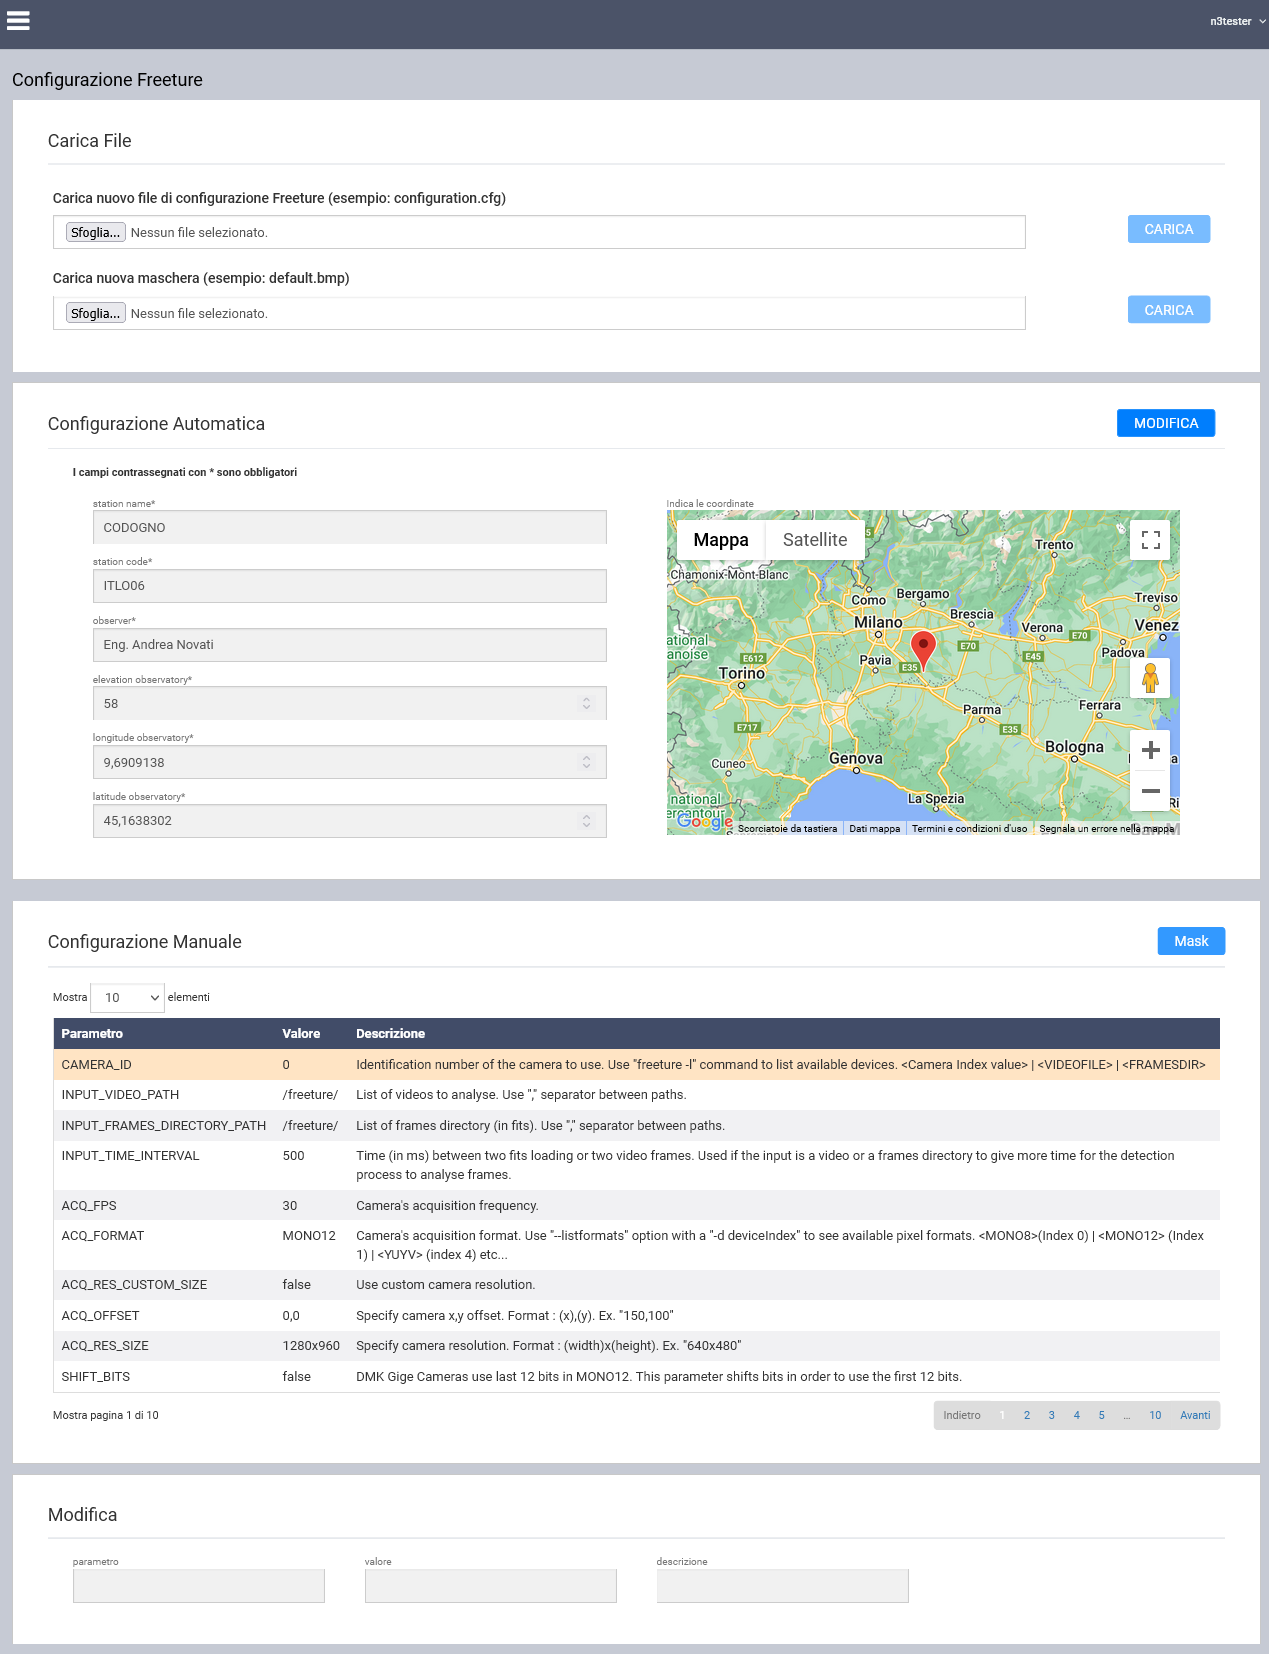
\includegraphics[width=\textwidth]{images/full-freeture.png}
    \caption{Sezione \emph{Configurazione FreeTure}.}
    \label{fig:freeture}
    \end{center}
\end{figure}

\subsection{Caricamento nuova configurazione}

Si permette all'utente di caricare un file di \textbf{configurazione} completo di FreeTure, in formato \textbf{CONF}, mediante un apposito \textbf{\emph{file picker}}. Il server, una volta ricevuto il file, lo copia nel rispettivo volume \emph{freeture-conf} e riavvia il container (cfr. sezione \ref{docker}).

L'utente può anche decidere di caricare una \textbf{maschera} (cfr. sezione \ref{freeture}) in formato \textbf{BMP}, sempre tramite file picker. In questo caso, il server copierà la maschera nel volume \emph{freeture-data} (cfr. sezione \ref{docker}), opzionalmente modificando il file di configurazione esistente per selezionare la presenza di una nuova maschera.

Un messaggio di successo è mostrato se le operazioni sono andate a buon fine.

\begin{figure}[H]
    \begin{center}
    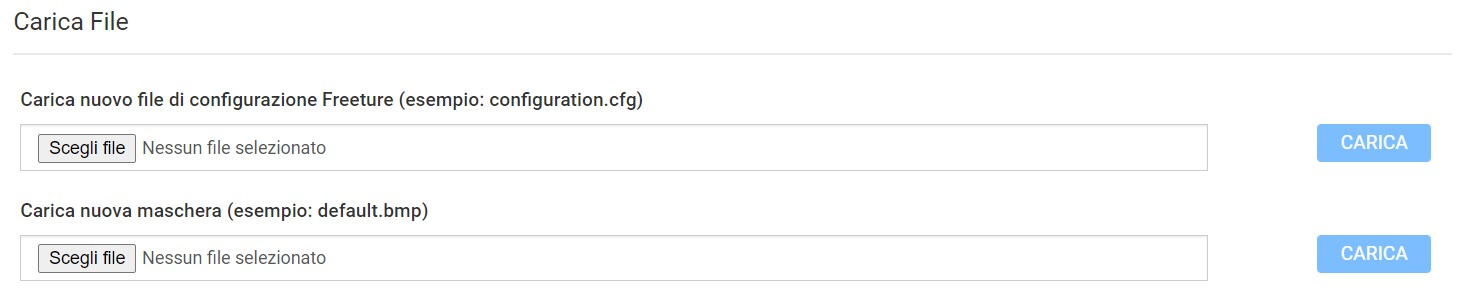
\includegraphics[width=\textwidth]{images/ft-carica-file.jpg}
    \caption{Caricamento file di configurazione o maschera.}
    \end{center}
\end{figure}

\subsection{Configurazione manuale}

Viene data la possibilità all'utente di modificare qualsiasi campo della configurazione; pertanto viene effettuato il parsing della configurazione dal server e visualizzato lato client con una tabella, realizzata tramite DataTables (cfr. sezione \ref{software}), le cui righe contengono \textbf{parametro}, \textbf{valore} e \textbf{descrizione} di ogni campo. Una volta cliccato sulla riga corrispondente, l'utente può modificare il valore del campo selezionato.
Un messaggio di successo è mostrato se l'operazione è andata a buon fine.

\begin{figure}[H]
    \begin{center}
    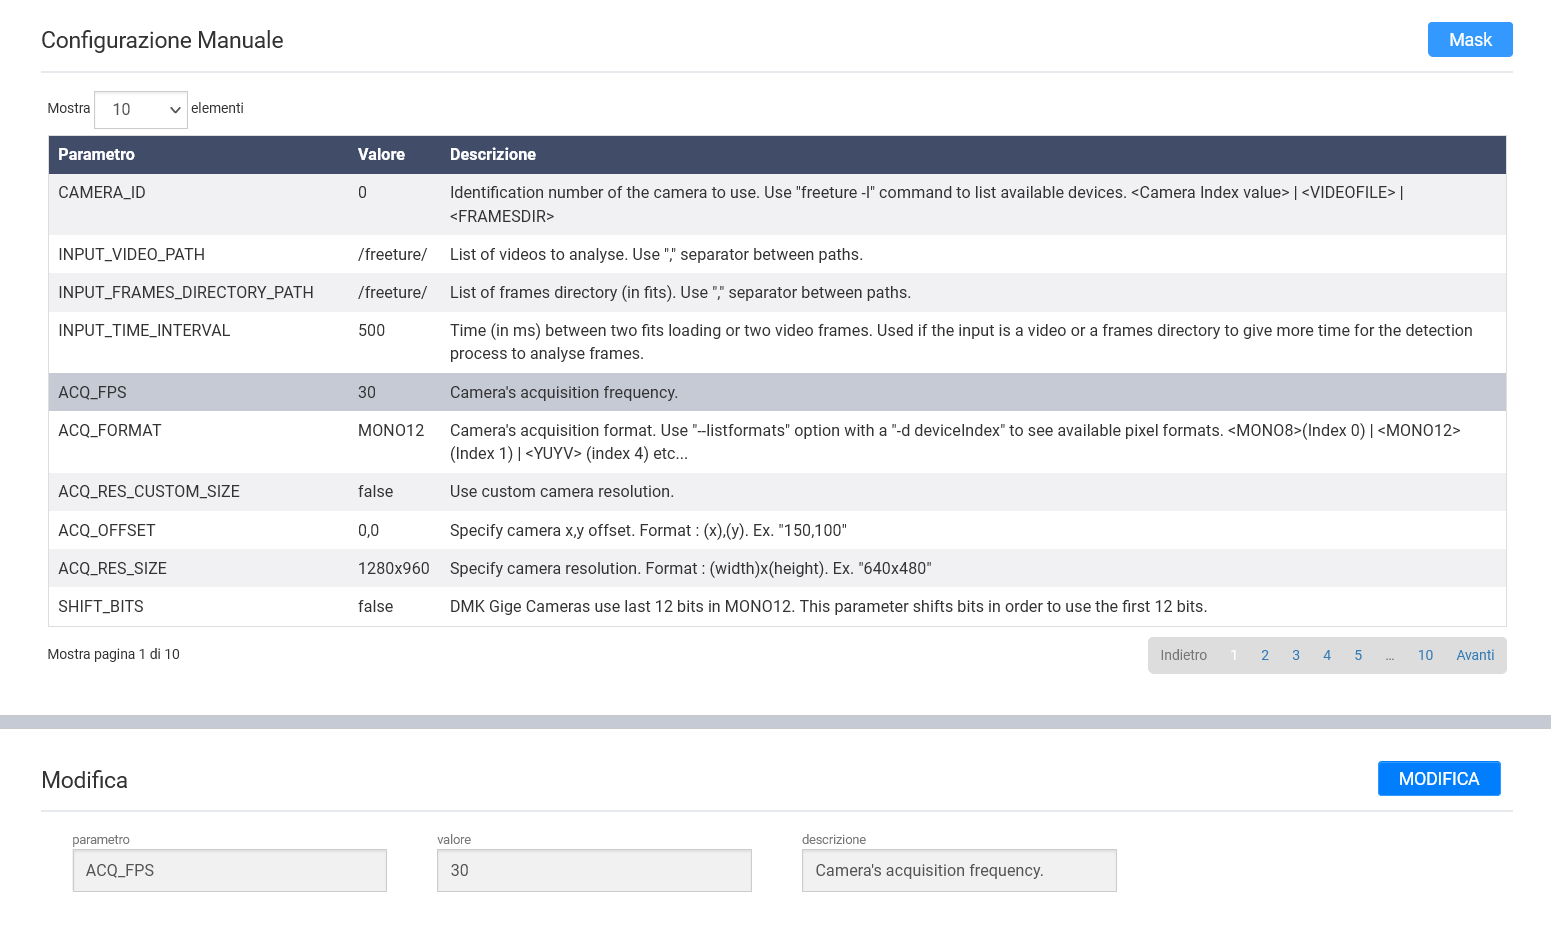
\includegraphics[width=\textwidth]{images/conf-manuale.png}
    \caption{Sezione di configurazione manuale. Sopra la tabella e sotto il campo di modifica del valore.}
    \end{center}
\end{figure}

\subsection{Configurazione automatica} \label{ft-conf-automatica}

Siccome, nella maggior parte dei casi, i principali campi oggetto di modifica sono ricorrenti e la modifica di un valore non è circoscritta ad un solo campo, l'utente può accedere ad una sezione di configurazione automatica, dove può modificare alcuni \textbf{valori chiave}. Le integrazioni a questi valori si ripercuotono poi su tutta la configurazione, andando a cambiare tutti i campi che sono coinvolti.

Una volta che la pagina web viene caricata, i campi in questione sono già precompilati con i valori correnti e l'utente può andare a cambiare solo quelli di suo interesse.

I campi sopracitati sono i seguenti:
\begin{itemize}
    \item \textbf{Nome della stazione}: solitamente è il nome della città dove si trova la stazione. È legato principalmente ai prefissi dei nomi dei file prodotti dalle elaborazioni astronomiche.
    \item \textbf{Codice della stazione}: è il codice univoco con cui si identifica la stazione. È coinvolto principalmente nei nomi delle cartelle generate da FreeTure.
    \item \textbf{Observer}: anagrafica della persona che gestisce la stazione.
    \item \textbf{Elevation observatory}: altitudine della stazione.
    \item \textbf{Longitude observatory}: longitudine della stazione.
    \item \textbf{Latitude observatory}: latitudine della stazione.
\end{itemize}

La web app si serve di un \textbf{sistema di validazione} dei campi degli input di tipo testo e numerico: all'utente non è ad esempio permesso lasciare un valore nullo. 

\begin{figure}[H]
    \begin{center}
    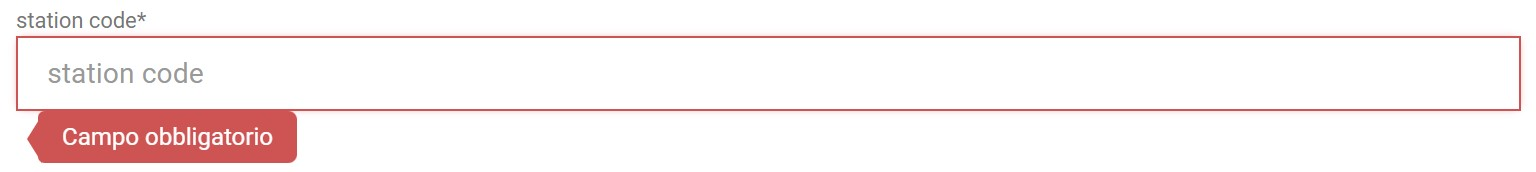
\includegraphics[width=\textwidth]{images/validator.jpg}
    \caption{Esempio di input improprio segnalato con un messaggio di errore.}
    \end{center}
\end{figure}

Inoltre, tramite l'utilizzo delle API di \textbf{GoogleMaps} (cfr. sezione \ref{software}), è stato realizzato un \textbf{\emph{location picker}}, grazie a cui l'utente può interagire con la mappa cliccando nel punto dove desidera localizzare la stazione, oppure avere un riscontro diretto dell'ubicazione delle coordinate inserite manualmente.

\begin{lstlisting}[style=JavaScript,caption={Parte dell'implementazione in JS per il \emph{location picker}.},captionpos=b,label={lst:location-picker}]
// Handle location picking
function changeMarkerLocation() {
    lat = Number($('#latitude-observatory').val());
    lng = Number($('#longitude-observatory').val());
    station = {lat: lat, lng: lng};
    if (marker === false) {
        marker = new google.maps.Marker({
            position: station,
            map: map,
            draggable: true
        });
        google.maps.event.addListener(marker, 'dragend', 
            function (event) {
                markerLocation();
            });
    } else {
        marker.setPosition(station);
    }
    map.setCenter({lat: lat, lng: lng});
}
\end{lstlisting}

\begin{figure}[H]
    \begin{center}
    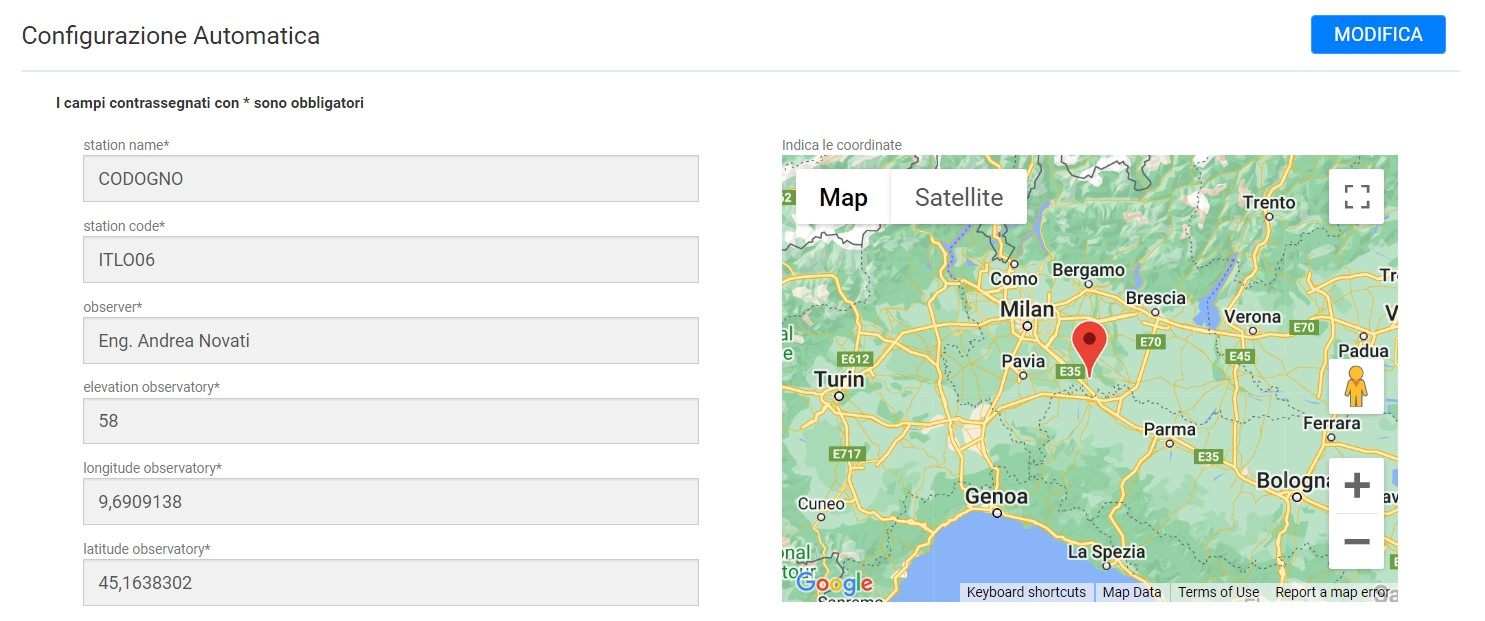
\includegraphics[width=\textwidth]{images/conf-automatica.jpg}
    \caption{Sezione di configurazione automatica. A destra il \emph{location picker} e a sinistra il campo di modifica del valore.}
    \end{center}
\end{figure}

\section{Sezione OpenVPN} \label{sezione-OVPN}
Accedendo alla \emph{Configurazione OpenVPN} (cfr. sezione \ref{rete-VPN}) nel menu, l'utente può effettuare due operazioni principali:

\begin{enumerate}[noitemsep,nolistsep]
    \item Caricare una nuova configurazione OpenVPN
    \item Visualizzare lo stato corrente della VPN
\end{enumerate}

\begin{figure}[H]
    \begin{center}
    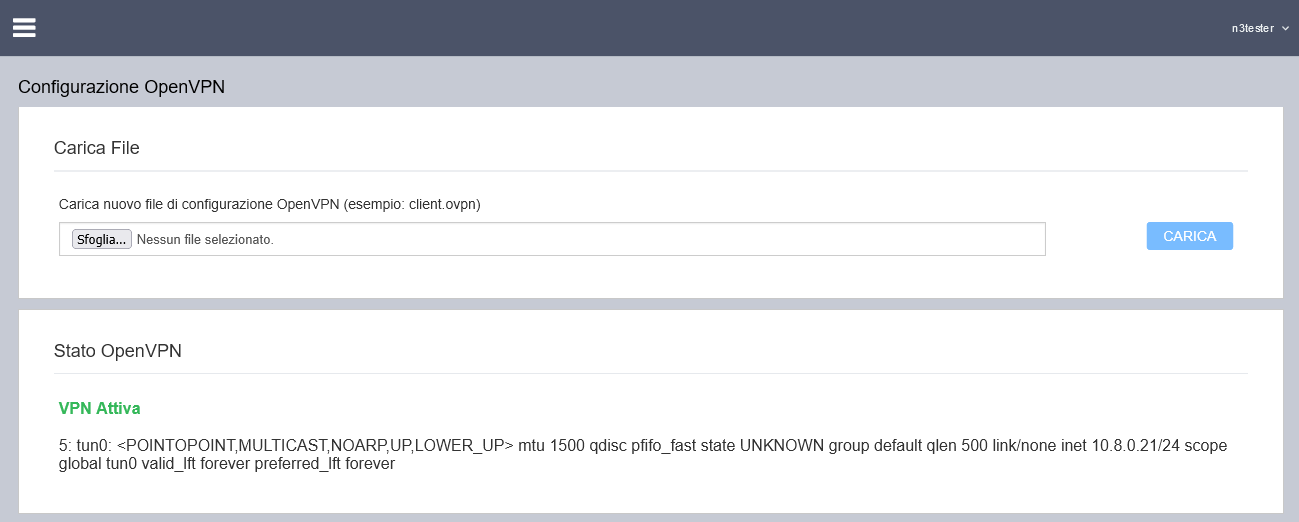
\includegraphics[width=\textwidth]{images/full-vpn.png}
    \caption{Sezione \emph{Configurazione OpenVPN}.}
    \end{center}
\end{figure}

\subsection{Caricamento nuova configurazione}

L'utente ha la possibilità di caricare un nuovo file di \textbf{configurazione OpenVPN} nell'apposita sezione, in formato \textbf{OVPN}. 

Quando il server riceve la nuova configurazione, deve prima di tutto \textbf{accedere in SSH} all'host dal container (cfr. sezione \ref{fig:containers-arch}); solo dopo essersi collegato al nodo può copiare il file di configurazione con SCP (\emph{Secure Copy}) e \textbf{riavviare la VPN}.

\begin{figure}[H]
    \begin{center}
    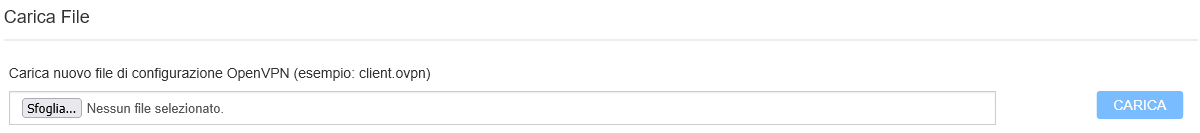
\includegraphics[width=\textwidth]{images/vpn-file.png}
    \caption{Sezione per il caricamento di un nuovo file di configurazione OpenVPN.}
    \end{center}
\end{figure}

\subsection{Visualizzazione stato corrente VPN}

Oltre a poter caricare una nuova configurazione, l'utente può visualizzare lo \textbf{stato corrente} della VPN sulla macchina.

\begin{figure}[H]
    \begin{center}
    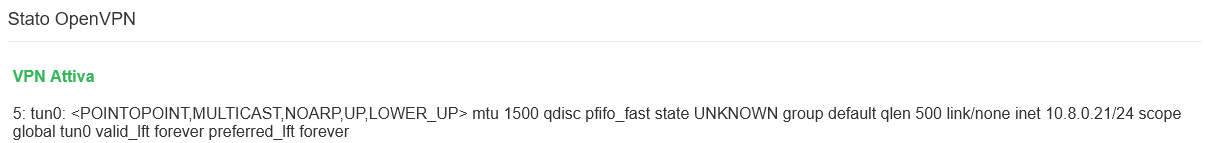
\includegraphics[width=\textwidth]{images/vpn-status.png}
    \caption{Stato corrente VPN.}
    \end{center}
\end{figure}

Per ottenere lo stato della VPN il server accede in SSH all'host e ricava le informazioni con il seguente comando eseguito nella shell:

\begin{verbatim}
    ip addr show dev tun0
\end{verbatim}

\section{Sezione Prometheus} \label{sezione-prometheus}
La sezione \emph{Configurazione Prometheus} (cfr. sezione \ref{prometheus}) selezionabile dal menu consente all'utente due operazioni essenziali:

\begin{enumerate}[noitemsep,nolistsep]
    \item Caricare una nuova configurazione Prometheus
    \item Visualizzare lo stato corrente della Prometheus
\end{enumerate}

\begin{figure}[H]
    \begin{center}
    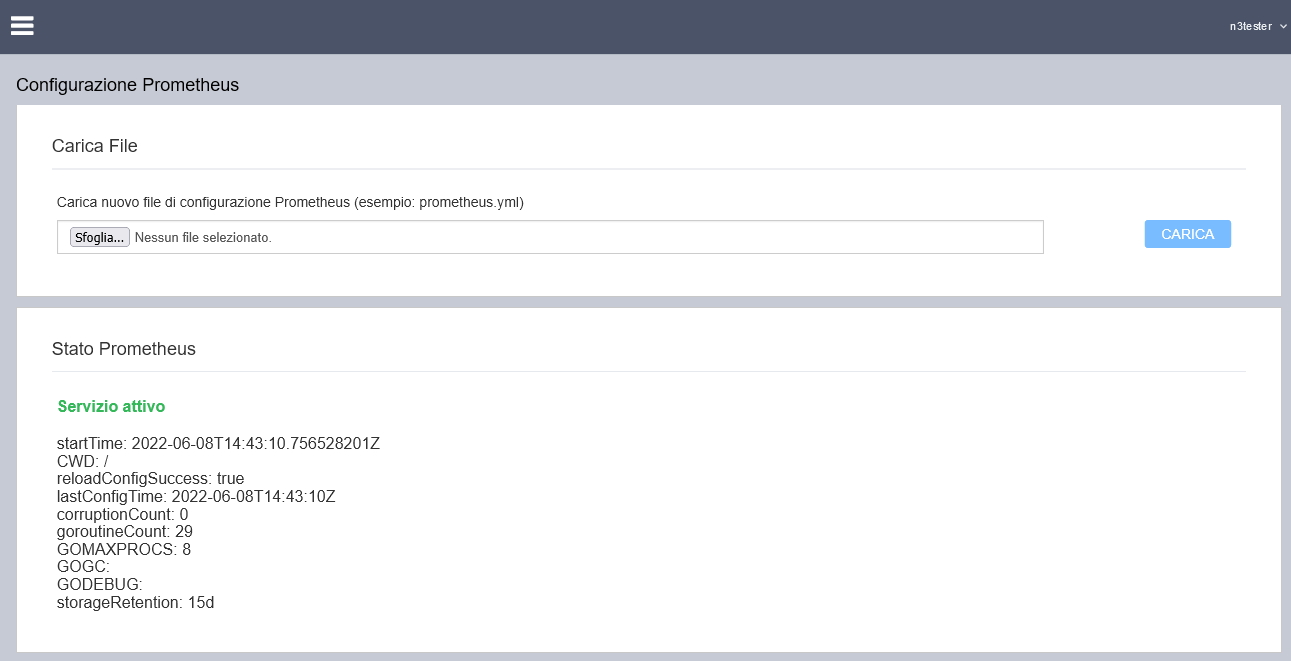
\includegraphics[width=\textwidth]{images/full-prometheus.png}
    \caption{Sezione \emph{Configurazione Prometheus}.}
    \end{center}
\end{figure}

\subsection{Caricamento nuova configurazione}

L'utente può caricare, in modo analogo alla sezione relativa alla VPN, un nuovo file di \textbf{configurazione Prometheus}, in formato \textbf{YML}. 

Ugualmente alla configurazione OpenVPN, il server al momento della ricezione del nuovo file, \textbf{accede in SSH} all'host dal container (cfr. sezione \ref{fig:containers-arch}); successivamente copia con SCP il nuovo file di configurazione e \textbf{riavvia il service Prometheus}.

\begin{figure}[H]
    \begin{center}
    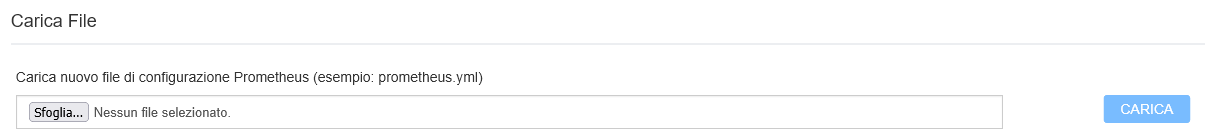
\includegraphics[width=\textwidth]{images/prometheus-file.png}
    \caption{Sezione per il caricamento di un nuovo file di configurazione OpenVPN.}
    \end{center}
\end{figure}

\subsection{Visualizzazione stato corrente Prometheus}

Come per la VPN, anche per Prometheus l'utente ha la facoltà di visualizzare lo \textbf{stato corrente} del servizio.

\begin{figure}[H]
    \begin{center}
    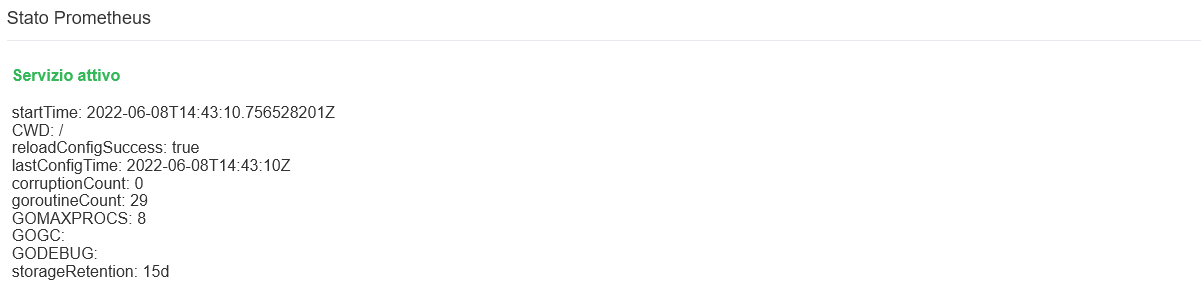
\includegraphics[width=\textwidth]{images/prometheus-status.png}
    \caption{Stato corrente Prometheus.}
    \end{center}
\end{figure}

La web application ricava lo stato di Prometheus direttamente dal client facendo una \emph{request} all'endpoint predefinito dal servizio:\\
\texttt{http://<hostname>:9090/api/v1/status/runtimeinfo}

\section{Sezione Container} \label{sezione-container}
Nella sezione \emph{Stato Containers} l'utente può prendere visione dell'elenco dei container sulla macchina e eseguire alcune operazioni su di essi.

\begin{figure}[H]
    \begin{center}
    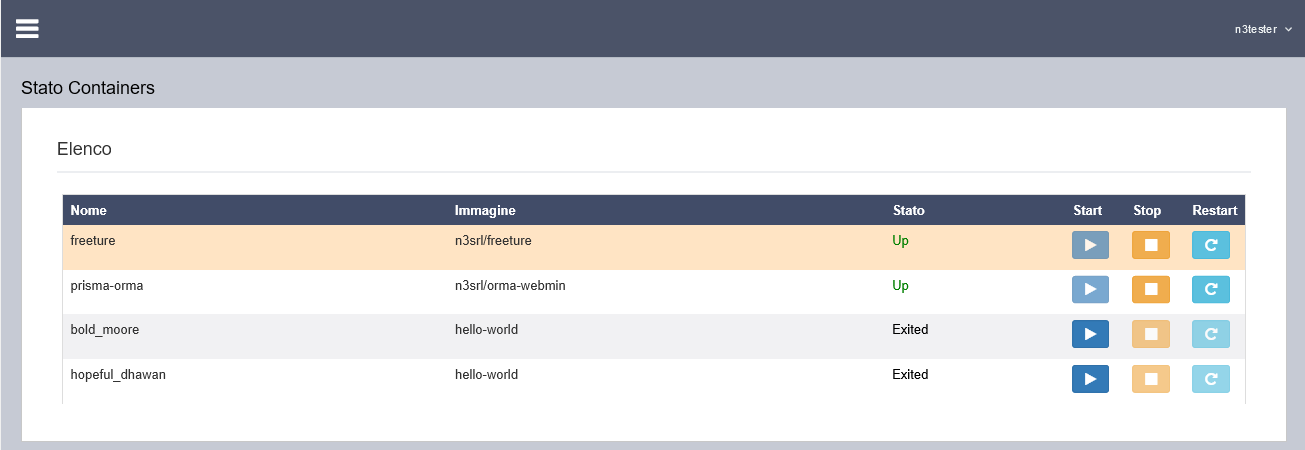
\includegraphics[width=\textwidth]{images/full-containers.png}
    \caption{Sezione \emph{Stato Containers}.}
    \end{center}
\end{figure}

\subsection{Visualizzazione container}

Nel dettaglio, i container sono organizzati in una tabella, realizzata con DataTables. Per ciascuno è riportato \textbf{nome del container}, \textbf{nome dell'immagine} e \textbf{stato corrente}. Gli stati possibili di un container sono:
\begin{itemize}[noitemsep,nolistsep]
    \item \emph{Up}: il container è attivo;
    \item \emph{Restarting}: il container si sta riavviando;
    \item \emph{Exited}: il container non è attivo.
\end{itemize}

\subsection{Avvio, riavvio e interruzione container}

L'utente ha la facoltà di interagire con i container elencati con tre pulsanti disponibili che consentono di:
\begin{itemize}[noitemsep,nolistsep]
    \item Avviare il container (\textbf{Start}), possibile solo se un container è fermo;
    \item Riavviare il container (\textbf{Restart}), possibile solo se un container è attivo o si sta riavviando;
    \item Fermare il container (\textbf{Stop}), possibile solo se un container è attivo o si sta riavviando.
\end{itemize}

I pulsanti inerenti a operazioni non possibili in quel momento risultano disattivati all'utente.

Il server per realizzare le richieste dell'utente deve prima accedere in SSH all'host dei container e solo successivamente eseguire i comandi Docker.

\section{Sezione Utenti} \label{sezione-utenti}
Nella sezione \emph{Utenti} è possibile visualizzare l'elenco di tutti gli utenti e cambiare la password corrispondente.

\begin{figure}[H]
    \begin{center}
    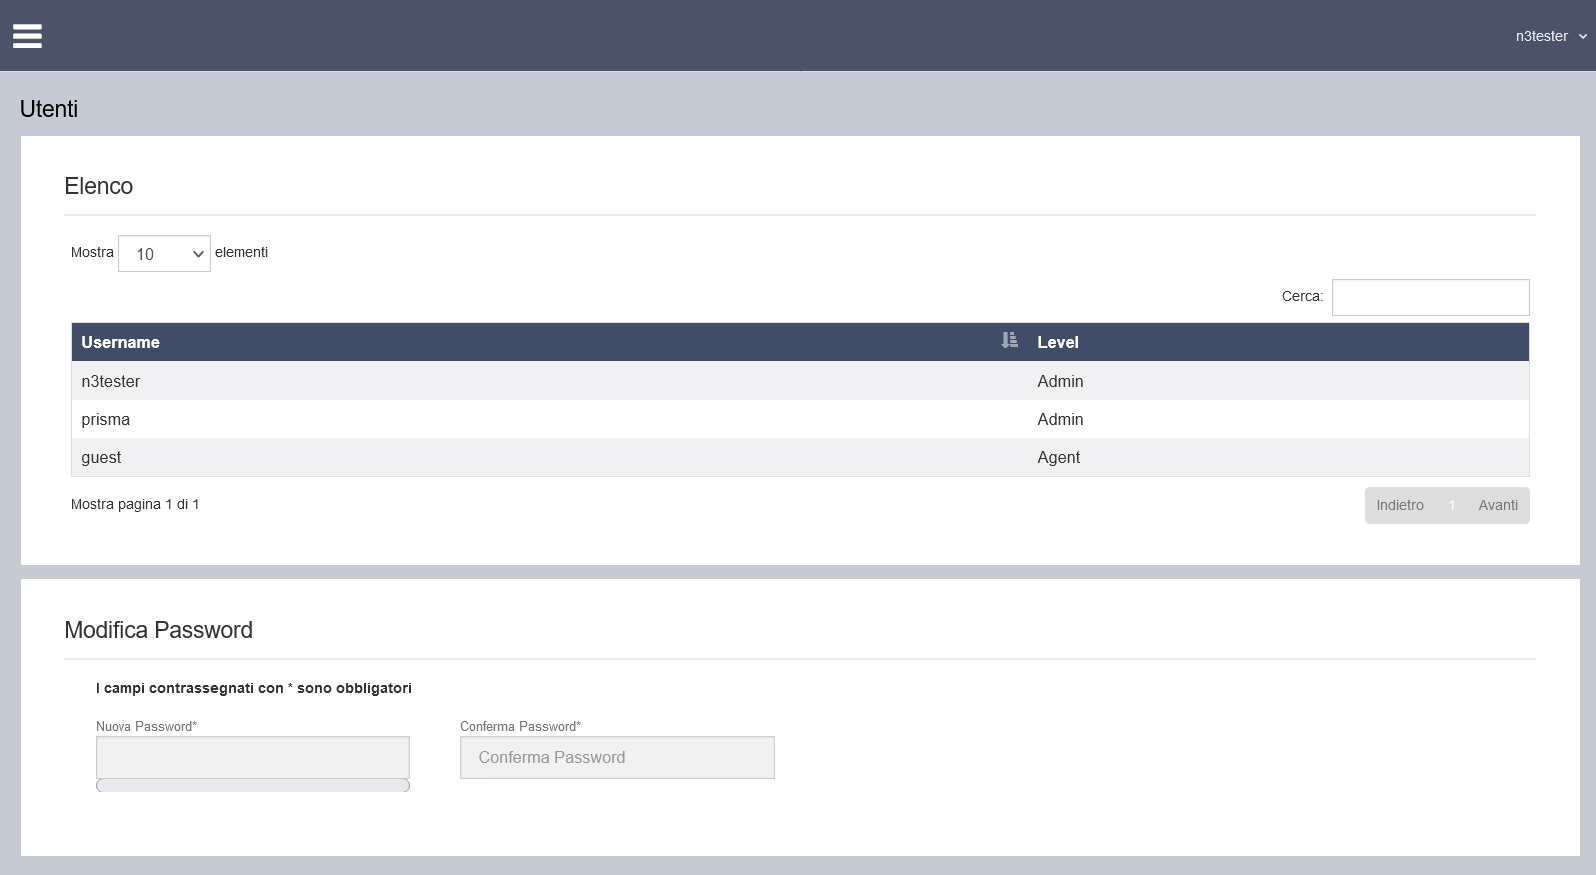
\includegraphics[width=\textwidth]{images/full-utenti.png}
        \caption{Sezione \emph{Utenti}.}
    \end{center}
\end{figure}

\subsection{Visualizzazione utenti}

La pagina mostra una tabella, implementata con DataTables, con l'elenco degli username di tutti gli utenti che possono accedere al sistema e il rispettivo livello (cfr. sezione \ref{sicurezza}).

\subsection{Cambio password}

\begin{wrapfigure}{l}{0.3\textwidth}
    \vspace{-4pt}
    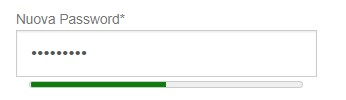
\includegraphics[width=0.3\textwidth]{images/pwd-strength-meter.jpg}
    \vspace{-24pt}
\end{wrapfigure}

Cliccando sulla relativa riga, si può accedere al cambio della password. Similmente ai campi nella configurazione automatica di Freeture (cfr. sezione \ref{ft-conf-automatica}), la password è gestita da un \textbf{sistema di validazione} e sottoposta ad un \textbf{controllo di robustezza} (\emph{strength meter}).

\subsection{Gestione sicurezza} \label{sicurezza}

Per rendere più sicura la web application dal momento che si interagisce con dati sensibili sul nodo, durante il lavoro è stato introdotto un sistema di sicurezza associato ai privilegi degli utenti. 

Come già accennato, ad ogni utente corrisponde un certo \textbf{livello}. I livelli possibili sono:
\begin{itemize}[noitemsep,nolistsep]
    \item \textbf{Admin}: livello amministratore, l'utente ha accesso a tutte le sezioni;
    \item \textbf{Agent}: livello base, l'utente ha accesso solo ad alcune sezioni non amministrative ma solo di consultazione.
\end{itemize}

Un utente \emph{Agent} condivide con gli amministratori solo la homepage e le  sezioni \emph{Calibrazioni}, \emph{Stack} e \emph{Detection}. Inoltre ha accesso alla sezione \emph{Configurazione FreeTure} (cfr. sezione \ref{sezione-freeture}) sebbene ridotta (cfr. figura \ref{fig:freeture-ridotto}), dove può solamente modificare l'anagrafica dell'\emph{observer} associato alla stazione.

Qualora un utente cerchi di accedere tramite URL a pagine non autorizzate, viene reindirizzato alla pagina di login.

\begin{figure}[H]
    \begin{center}
    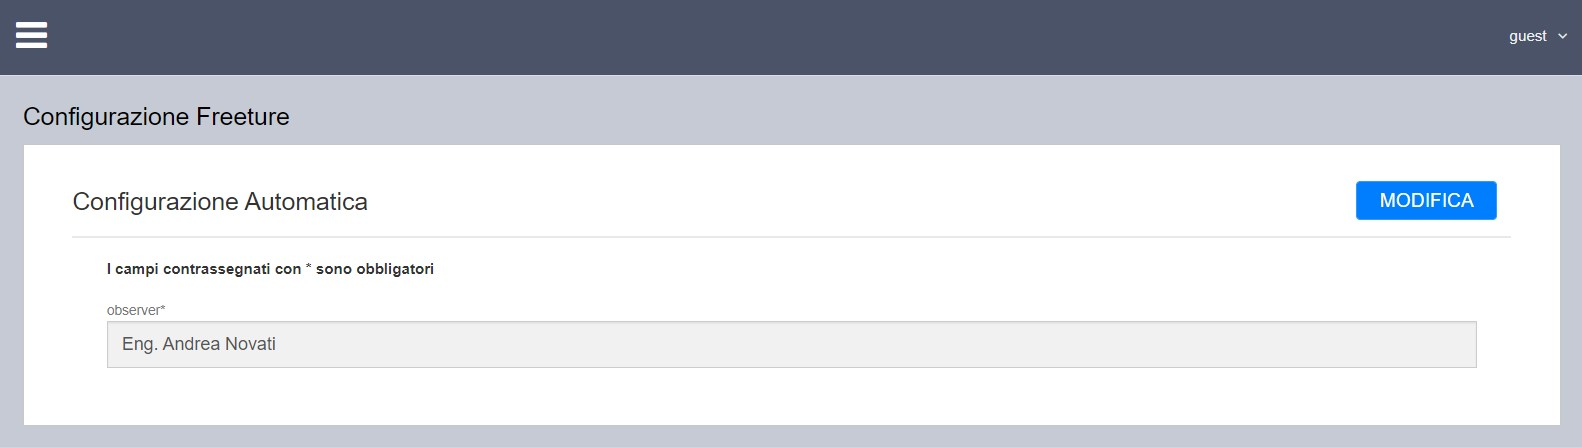
\includegraphics[width=\textwidth]{images/freeture-ridotto.jpg}
    \caption{Sezione \emph{Configurazione FreeTure} per gli utenti di livello \emph{Agent}.}
    \label{fig:freeture-ridotto}
    \end{center}
\end{figure}

\begin{figure}
    \begin{center}
    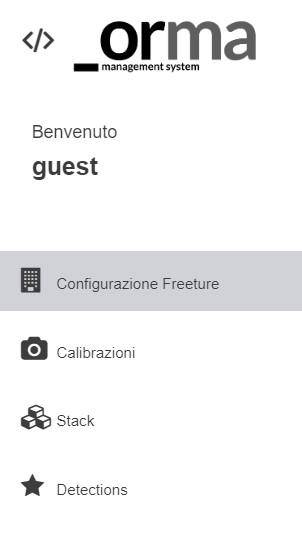
\includegraphics[width=0.4\textwidth]{images/menu-ridotto.jpg}
        \caption{Menu della web application per gli utenti di livello \emph{Agent}.}
        \label{fig:menu-ridotto}
    \end{center}
\end{figure}



\section{Sezione Capture e Stack} \label{sezione-capture-stack}
Tutti gli utenti, a prescindere dal livello, possono consultare i dati raccolti dal nodo (cfr. \ref{dati-raccolti}) in tre sezioni principali:
\begin{itemize}[noitemsep,nolistsep]
    \item Calibrazioni (o Capture)
    \item Stack
    \item Detection
\end{itemize}

Nella sezione corrente verranno trattate insieme le prime due (cfr. figure \ref{fig:calibrazioni} e \ref{fig:stack}), dal momento che sono analoghe eccetto per i dati.

\subsection{Visualizzazione dati raccolti} \label{capture-struct}

Sia le calibrazioni che gli stack sono organizzati in una struttura tabellare analoga a quella delle cartelle sul nodo (cfr. \ref{dati-raccolti}). La \textbf{prima tabella} contiene l'elenco dei \textbf{giorni}, dieci per pagina, e il numero delle calibrazioni o degli stack di quel giorno. La \textbf{seconda tabella} mostra invece le calibrazioni o gli stack del giorno selezionato sulla prima tabella, anche in questo caso dieci per pagina. Ciascuna riga contiene \textbf{nome della calibrazione/stack}, l'\textbf{ora} in cui è stata catturata l'immagine e due pulsanti, \textbf{Anteprima} e \textbf{Download} (cfr. figura \ref{fig:capture-table}). Sotto le tabelle è mostrata l'\textbf{ultima immagine rilevata} e relativa didascalia.

\begin{wrapfigure}{r}{0.3\textwidth}
    \vspace{-30pt}
    
\includegraphics[width=0.3\textwidth]{images/toggle-button.jpg}
    \vspace{-30pt}
\end{wrapfigure}
Il pulsante \textbf{Download} permette di scaricare il \textbf{file FITS} dell'immagine ed è sempre abilitato.
Il pulsante \textbf{Anteprima} mostra invece a schermo in una \textbf{finestra modale} l'immagine convertita in \textbf{PNG} in modo da poterla visualizzare (cfr. figura \ref{fig:capture-preview}). Si noti che questo pulsante è disabilitato di default: per porterlo abilitare è necessario attivare il \textbf{\emph{toggle button}} in alto a destra. Una volta attivato, l'utente dovrà aspettare una manciata di secondi, dal momento che il server si occupa di convertire tutte e dieci le immagini (cfr. sezione \ref{elaborazione-dati-capture}) che vengono poi mandate al client in codifica \emph{Base64} e memorizzate in locale. Il \emph{toggle button} è stato pensato per non appesantire l'esperienza dell'utente nello scorrere le pagine della tabella con inutili caricamenti.
Per implementare questa funzionalità si è fatto un largo uso dell'implementazione server-side di \textbf{DataTables}.

\begin{figure}[H]
    \begin{center}
    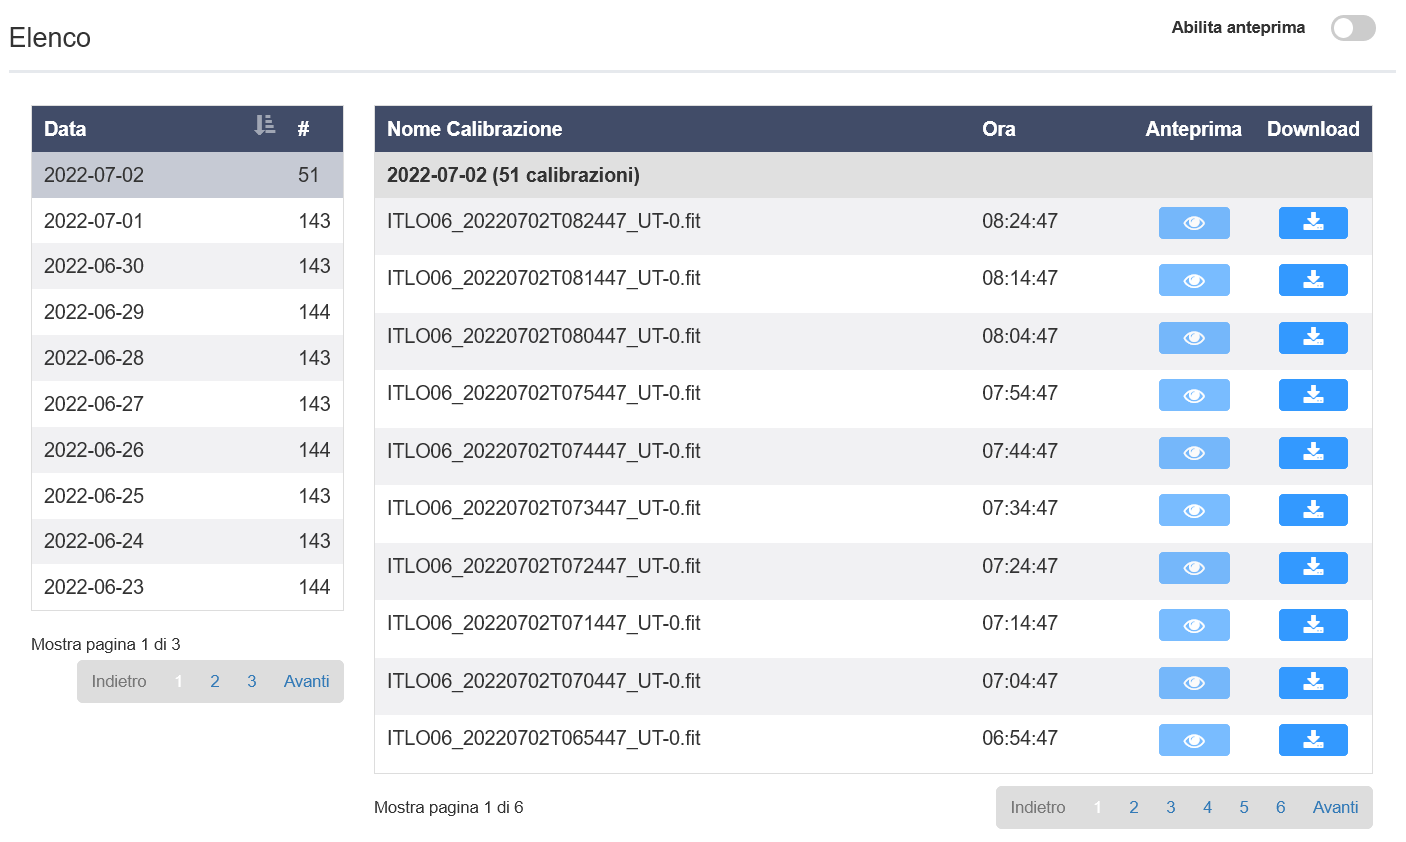
\includegraphics[width=\textwidth]{images/captures-table.png}
    \caption{Visualizzazione elenco calibrazioni di un giorno.}
    \label{fig:capture-table}
    \end{center}
\end{figure}
\vspace{-24pt}
\begin{figure}[H]
    \begin{center}
    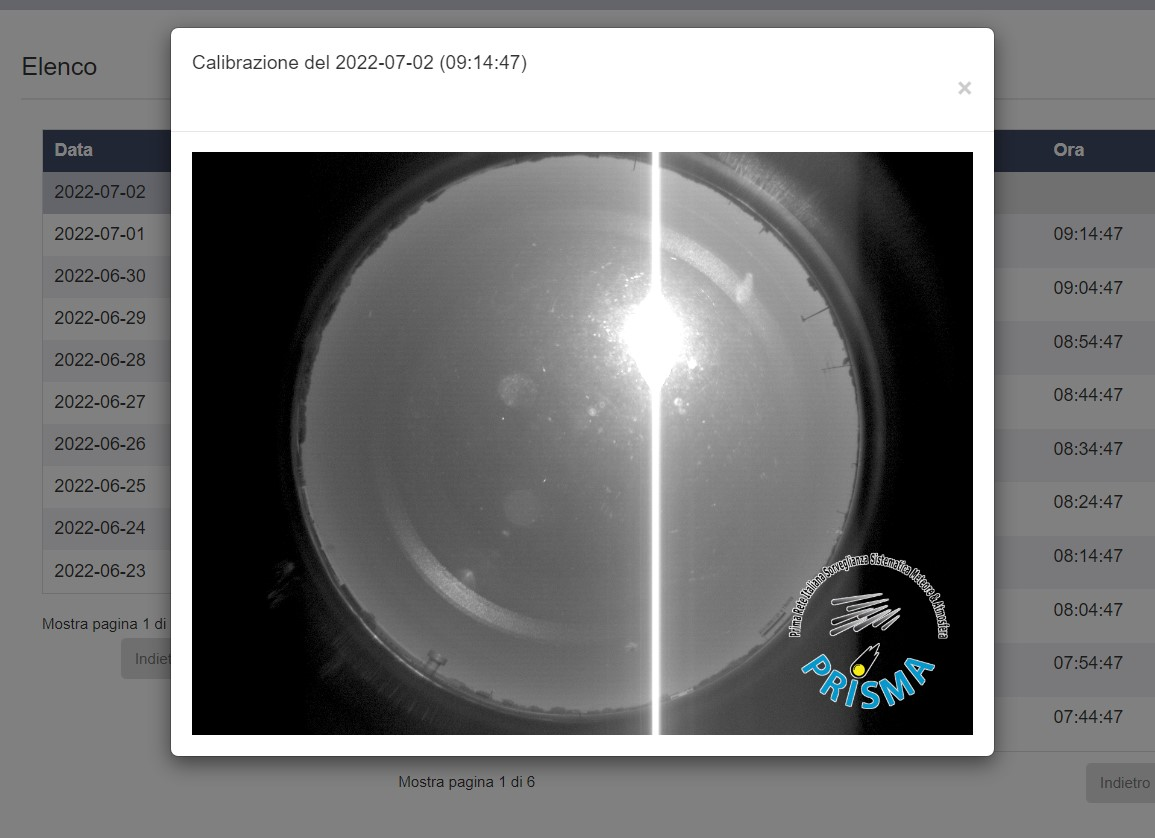
\includegraphics[width=\textwidth]{images/capture-preview.jpg}
    \caption{Anteprima di una calibrazione.}
    \label{fig:capture-preview}
    \end{center}
    
\end{figure}

\subsection{Elaborazione dei dati server-side} \label{elaborazione-dati-capture}

Quando l'utente abilita il \emph{toggle button}, oppure cambia pagina quando è attivo, il server si occupa di elaborare ciascuno dei dieci file consultabili in modo da rendere disponibile la visualizzazione dell'immagine lato client: il browser altrimenti non avrebbe modo di renderizzare il formato FITS.

L'elaborazione di ciascun file attraversa tre stadi:

\begin{enumerate}
    \item \textbf{Conversione in PNG}: il file FITS viene convertito in formato PNG mediante il software \textbf{fitspng} (cfr. sezione \ref{software});
    \begin{verbatim}
        fitspng -o <output_file> <input_file>
    \end{verbatim}
    \item \textbf{Watermarking}: all'immagine convertita viene aggiunto il logo del progetto PRISMA in basso a destra, servendosi di \textbf{ImageMagick} (cfr. sezione \ref{software});
    \begin{verbatim}
        composite -gravity SouthEast <logo> \ 
            <input_image> <output_image>
    \end{verbatim}
    \item \textbf{Conversione in \emph{Base64}}: il file ottenuto viene infine codificato in \emph{Base64} (cfr. listing \ref{lst:base64-coding}) .
\end{enumerate}

Si noti che tutti i file vengono temporaneamente salvati in una cartella di webroot e poi, una volta codificati in \emph{Base64} vengono eliminati per non occupare ulteriore spazio.

\begin{lstlisting}[style=PHP,caption={Metodo PHP per codificare i file in \emph{Base64}.},captionpos=b,label={lst:base64-coding}]
    // Encode image to base64
    public static function encodeCapture($path) {
        if (!file_exists($path)) {
            return "";
        }
        $data = file_get_contents($path);
        $base64 = 'data:image/png;base64,' . 
            base64_encode($data);
        return $base64;
    }
\end{lstlisting}

\begin{figure}[H]
    \begin{center}
    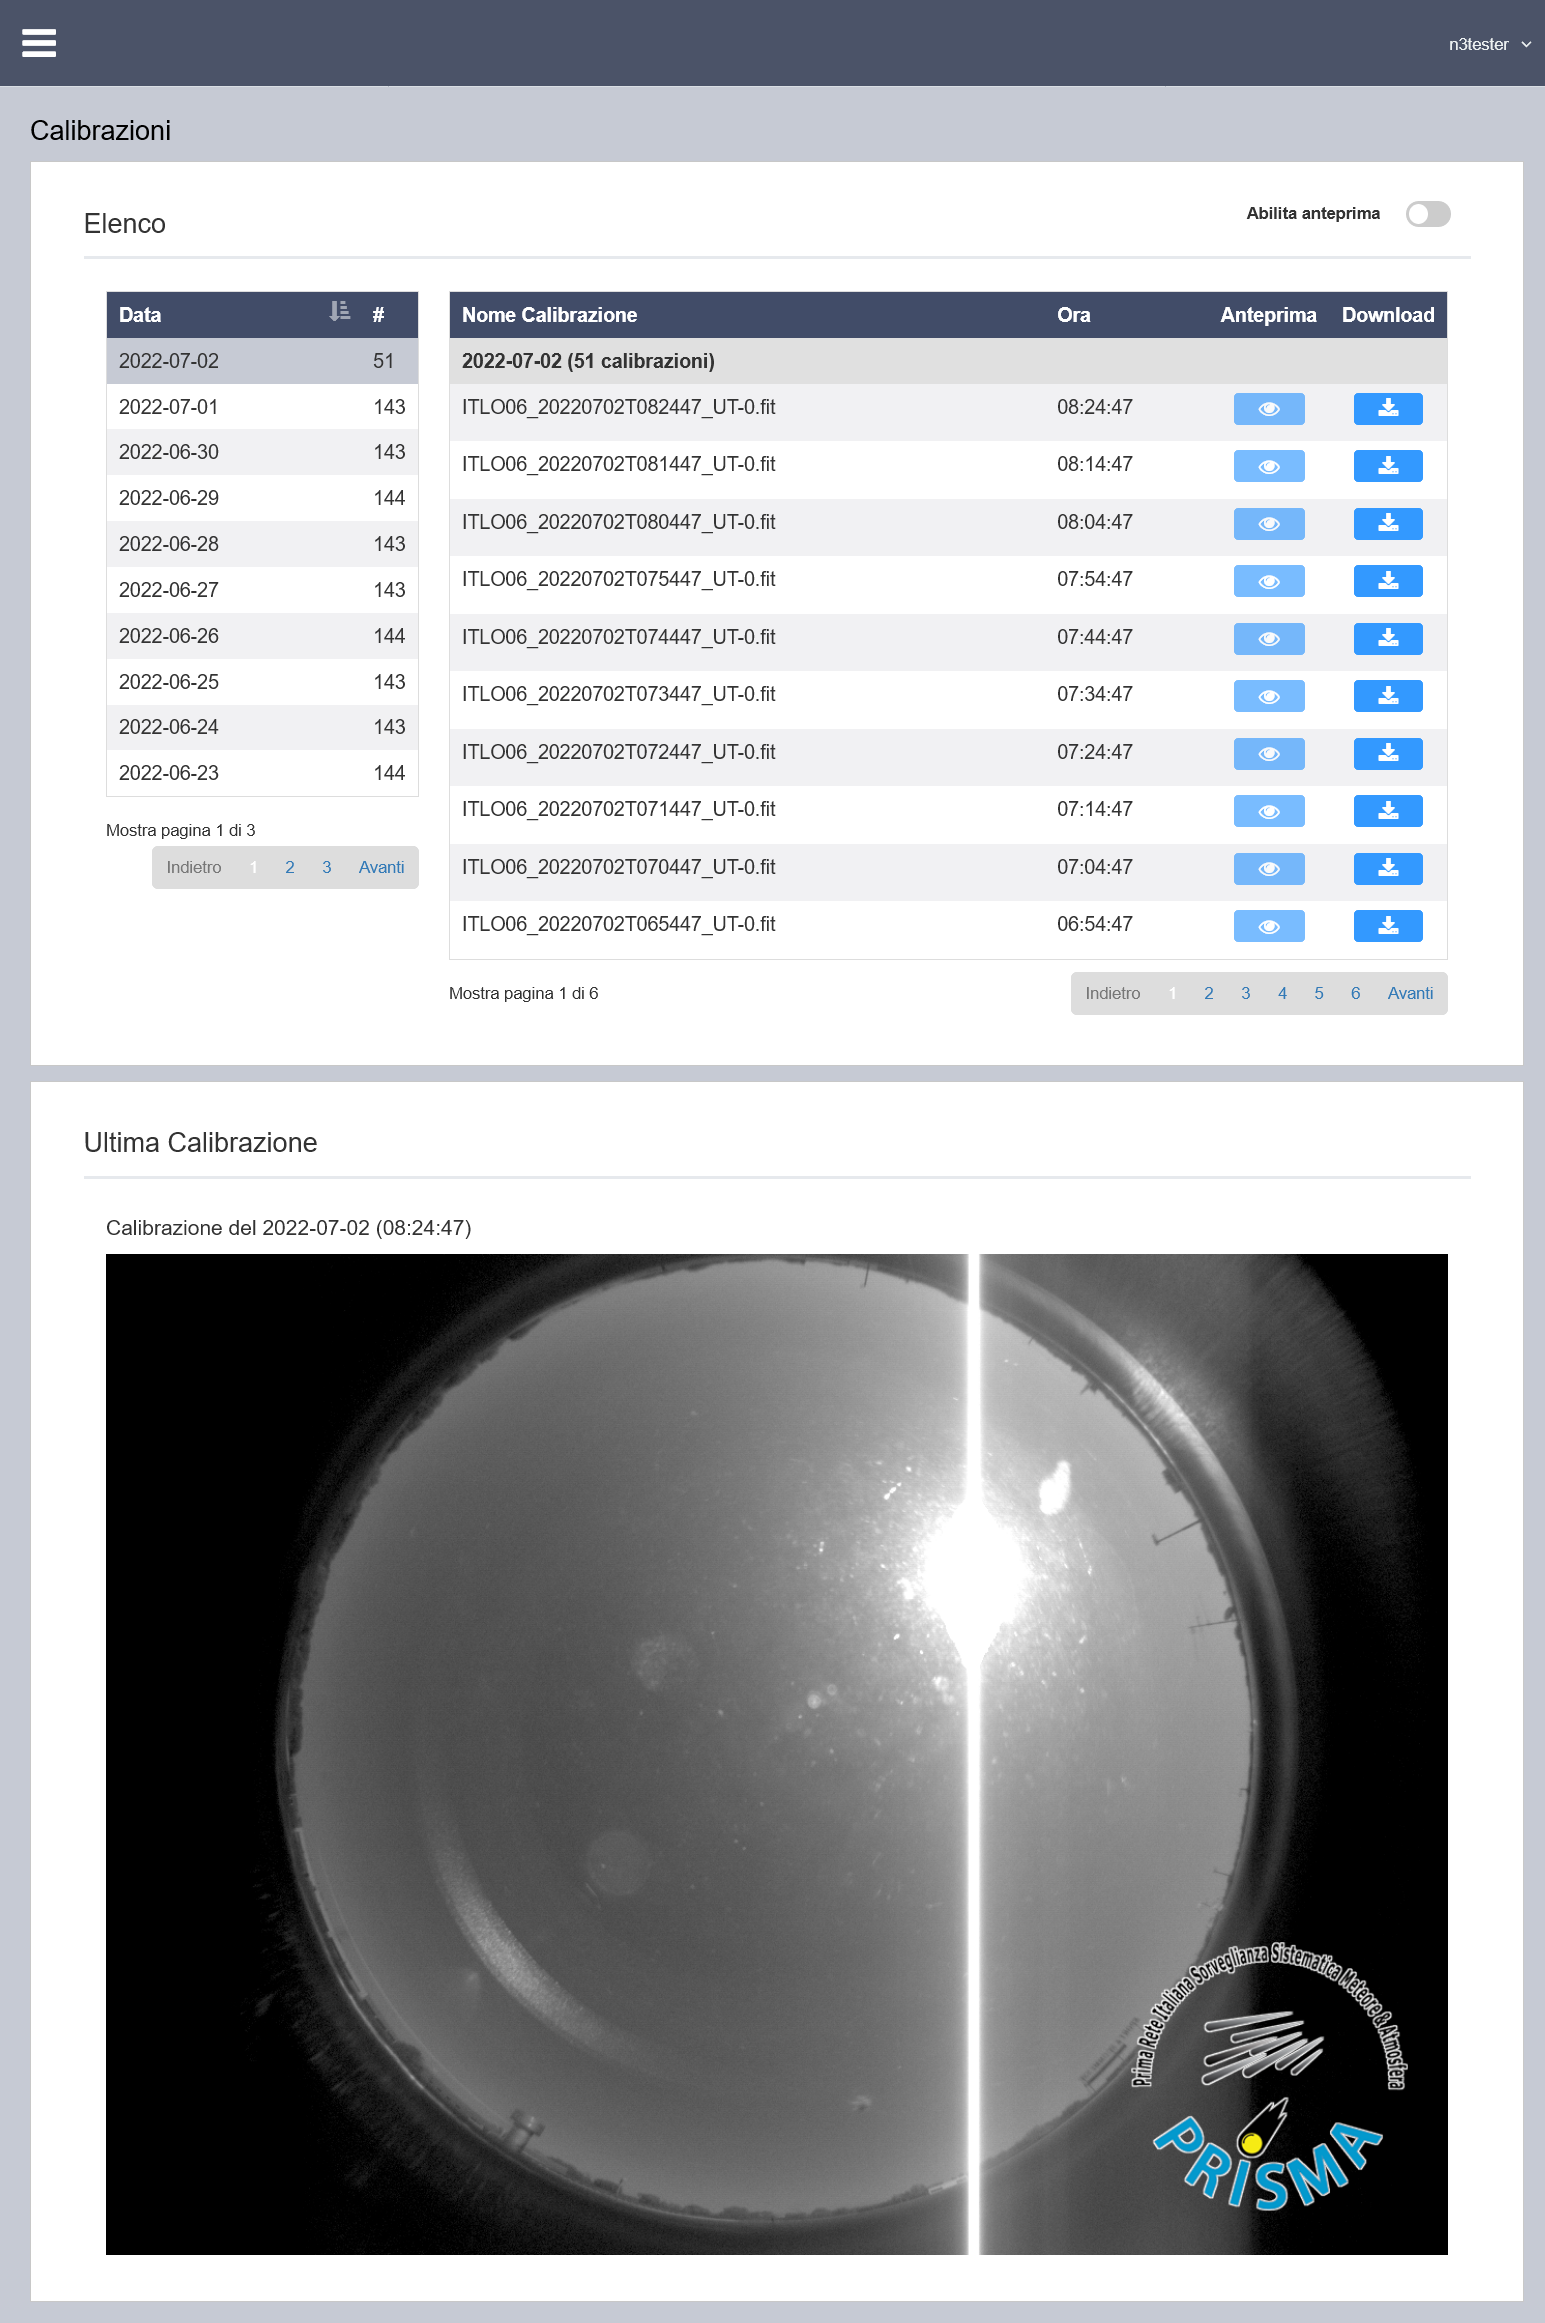
\includegraphics[width=\textwidth]{images/full-captures.png}
    \caption{Sezione \emph{Calibrazioni}.}
    \label{fig:calibrazioni}
    \end{center}
\end{figure}

\begin{figure}[H]
    \begin{center}
    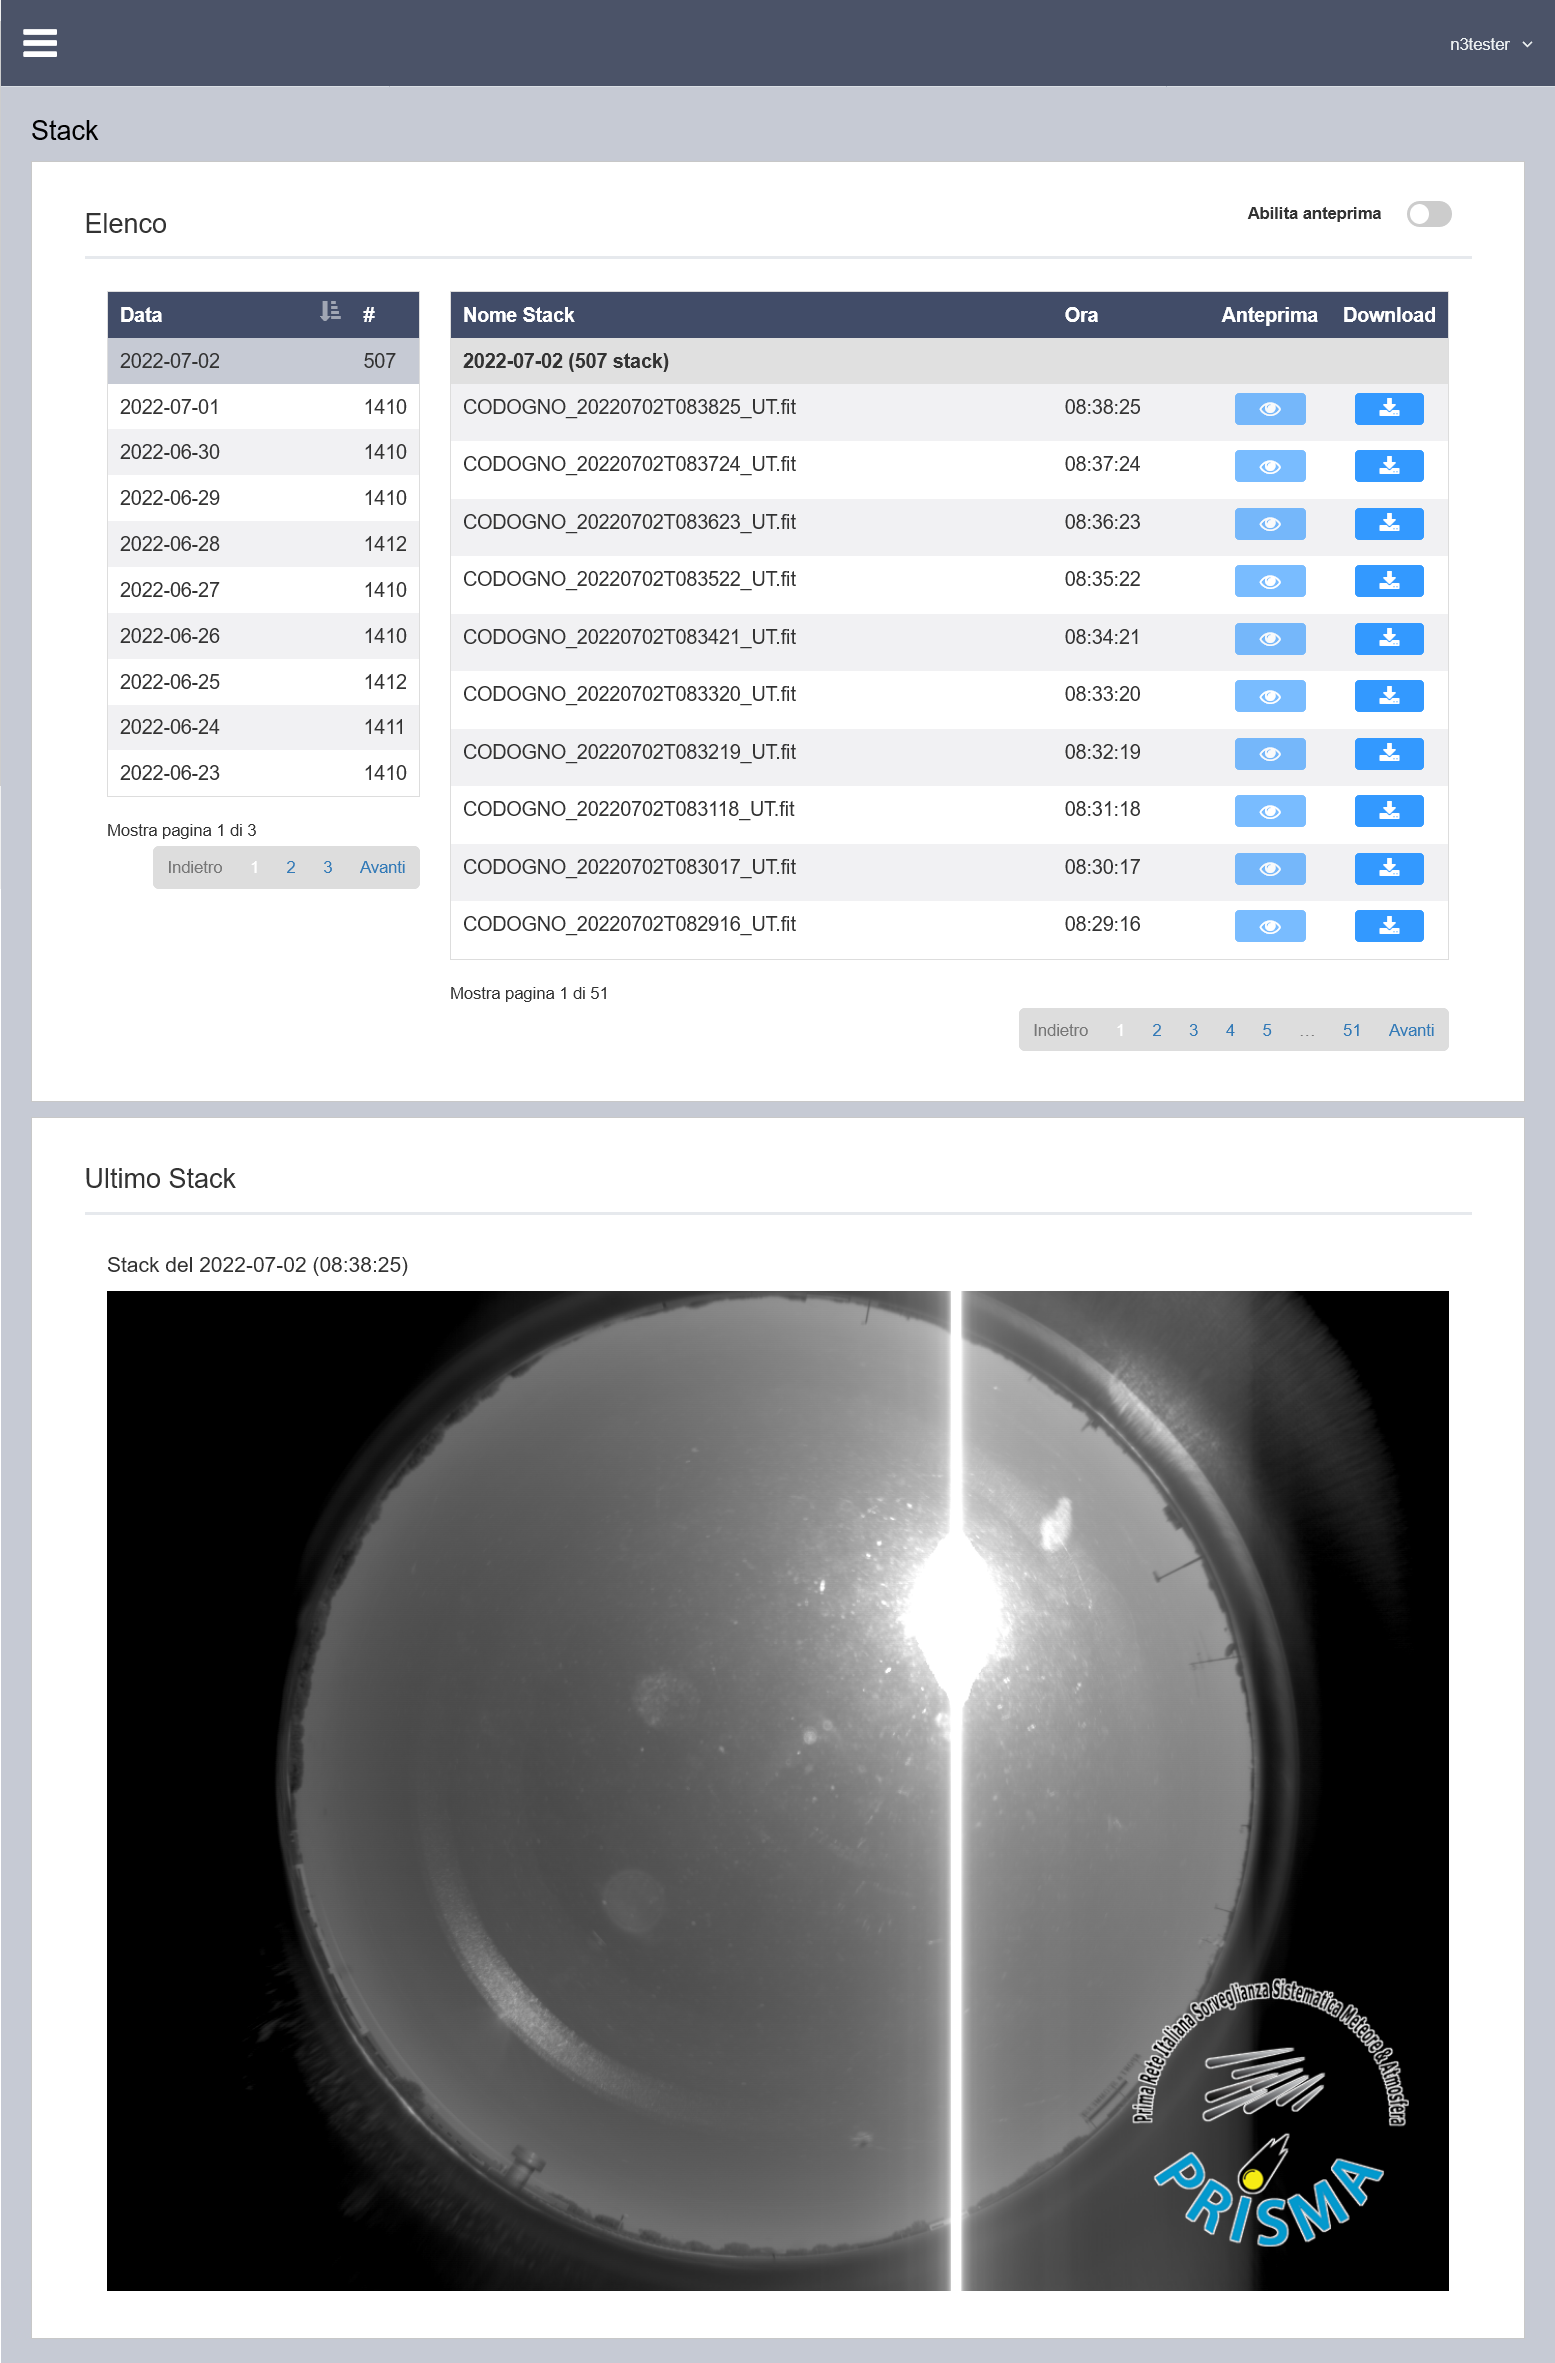
\includegraphics[width=\textwidth]{images/full-stacks.png}
    \caption{Sezione \emph{Stack}.}
    \label{fig:stack}
    \end{center}
\end{figure}

\section{Sezione Detection} \label{sezione-detection}
La terza sezione di consultazione dei dati raccolti è quella relativa alle detection (cfr. sezione \ref{dati-raccolti}).

\begin{figure}[H]
    \begin{center}
    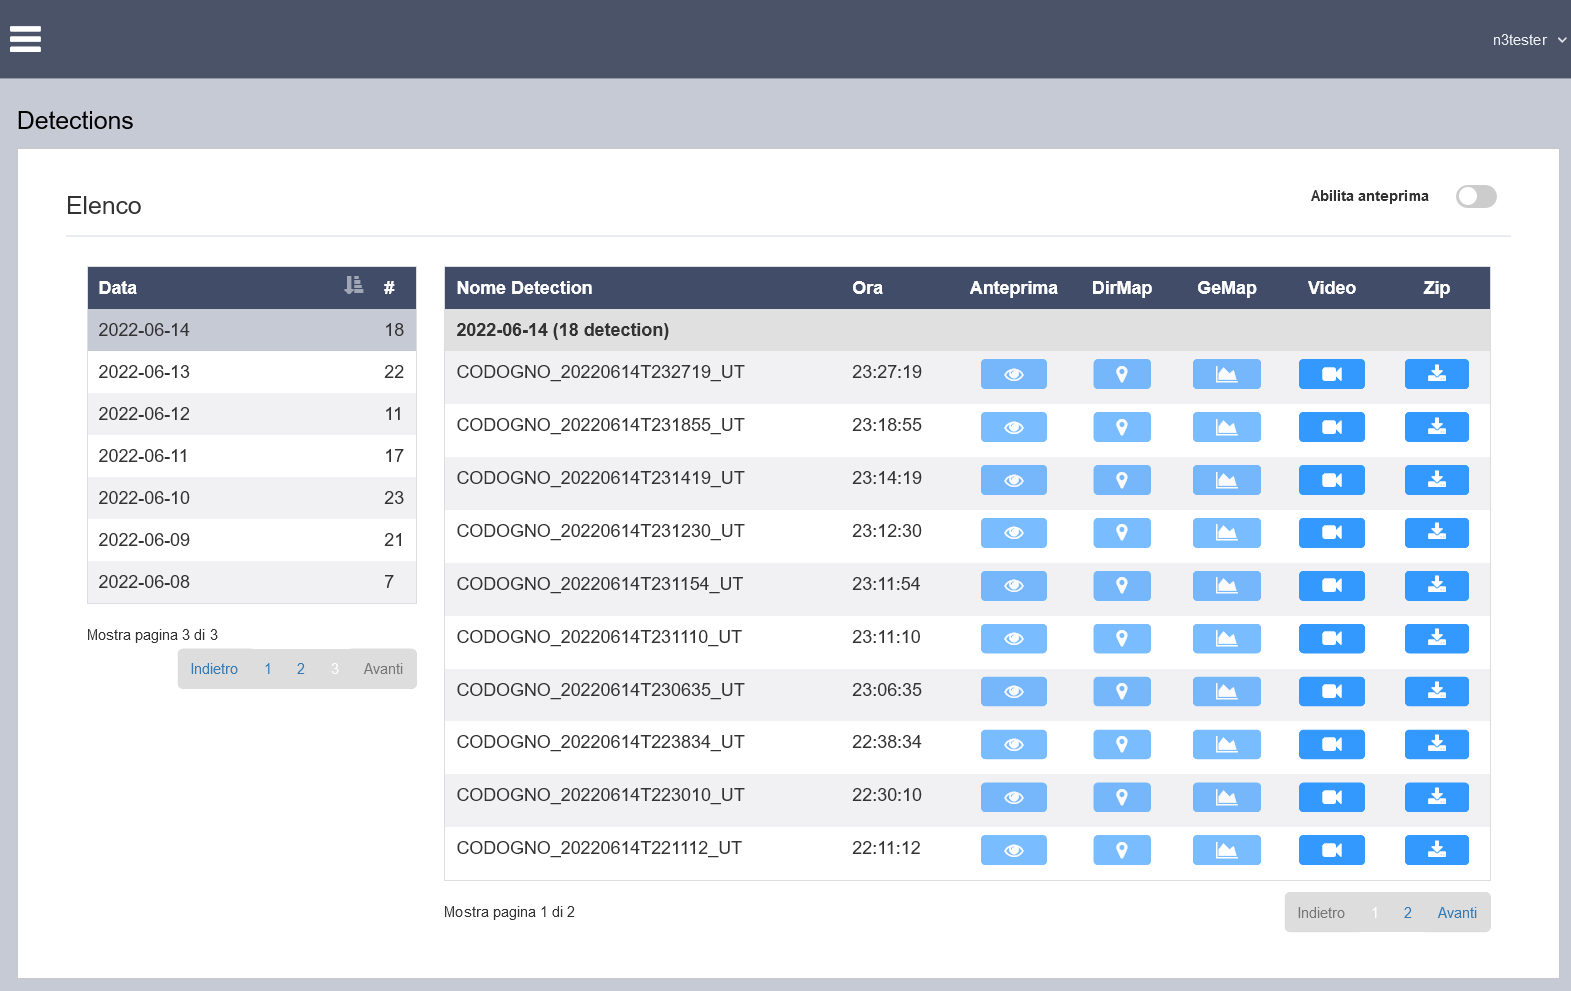
\includegraphics[width=\textwidth]{images/full-detection.png}
    \caption{Sezione \emph{Detection}.}
    \label{fig:detection}
    \end{center}
\end{figure}

\subsection{Visualizzazione dati raccolti} \label{detec-tables}

I dati sono articolati in una doppia tabella analoga a quella delle sezioni \emph{Capture} e \emph{Stack} (cfr. sezione \ref{capture-struct}). Per ogni giorno la seconda tabella mostra l'elenco delle \emph{detection} rilevate, con il nome della cartella, l'ora di rilevazione e cinque pulsanti di interazione: \textbf{Anteprima}, \textbf{DirMap}, \textbf{GeMap}, \textbf{Video} e \textbf{Zip}. È inoltre visibile l'immagine dell'ultima detection rilevata.

\begin{wrapfigure}{r}{0.3\textwidth}
    \vspace{-30pt}
    
\includegraphics[width=0.3\textwidth]{images/toggle-button.jpg}
    \vspace{-30pt}
\end{wrapfigure}
I pulsanti \textbf{Anteprima}, \textbf{DirMap} e \textbf{GeMap} si comportano in modo analogo a quello delle sezioni \emph{Capture} e \emph{Stack}, attivabili dal \textbf{\emph{toggle button}} \emph{Abilita anteprima}. Se cliccati, mostrano in una finestra modale il frame principale della rilevazione convertito in PNG (\emph{Anteprima}) e le immagini BMP DirMap e GeMap (cfr. sezione \ref{dati-raccolti}). Anche in questo caso, la conversione lato server delle immagini di anteprima risulterà in un'attesa di qualche secondo da parte dell'utente.

\begin{figure}[H]
    \begin{center}
    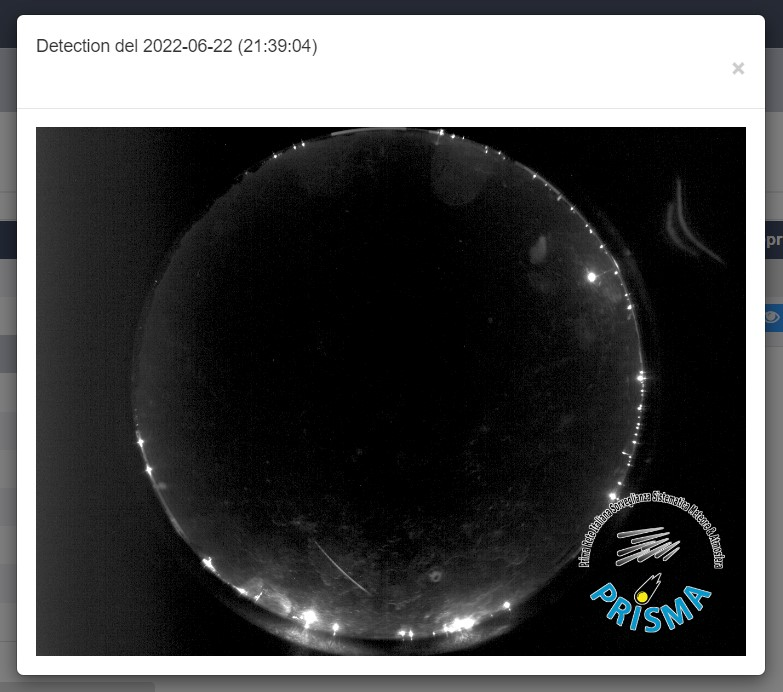
\includegraphics[width=\textwidth]{images/detec-preview.jpg}
    \caption{Anteprima della detection del 22/06/2022.}
    \end{center}
\end{figure}

Cliccando il pulsante \textbf{Video} viene invece scaricato il video della detection, mentre il pulsante \textbf{Zip} richiede lo zip della cartella della detection con i file in essa contenuti. Siccome il processo di elaborazione dei video e degli zip lato server è molto lungo (cfr. sezione \ref{elaborazione-dati-detec}), le richieste sono asincrone e compare un messaggio che avvisa l'utente di attendere qualche minuto prima che avvenga il download.

Inoltre, sempre per il motivo sopracitato, l'utente ha la facoltà di interrompere l'elaborazione in corso cliccando su un pulsante ad hoc (cfr. figure \ref{stop-video} e \ref{stop-zip}) che manda al server una richiesta per interrompere tutti i processi in esecuzione e abortire la chiamata AJAX in modo tale che il client non aspetti la risposta.

Infine, durante la preparazione dello zip o del video vengono disabilitati tutti gli altri pulsanti per ottenere zip o video in modo da non appesantire il server.

\begin{figure}[H]
    \begin{center}
    
\includegraphics[width=\textwidth]{images/stop-video.jpg}
    \caption{Il pulsante rosso permette l'interruzione dell'elaborazione del video sul server.}
    \label{stop-video}
    \end{center}
\end{figure}
\vspace{-24pt}
\begin{figure}[H]
    \begin{center}
    
\includegraphics[width=\textwidth]{images/stop-zip.jpg}
    \caption{Il pulsante rosso permette l'interruzione dell'elaborazione dello zip sul server.}
    \label{stop-zip}
    \end{center}
\end{figure}

\subsection{Elaborazione dei dati server-side} \label{elaborazione-dati-detec}

La consultazione dei dati relativi alle detection impiega consistenti risorse sul server: è stato dunque necessario gestire il più efficientemente possibile l'elaborazione dei dati e i processi ad essi relativi.

\subsubsection{Elaborazione immagini}

L'elaborazione dell'immagine di \textbf{anteprima} corrisponde a quella effettuata con capture e stack, con la conversione in PNG, il watermarking e la codifica in \emph{Base64} (cfr. sezione \ref{elaborazione-dati-capture}).

Le immagini \textbf{DirMap} e \textbf{GeMap} vengono semplicemente codificate in \emph{Base64} e inviate al client.

\subsubsection{Elaborazione video}

La generazione del video attraversa i seguenti stadi:
\begin{enumerate}
    \item \textbf{Conversione dei frame da FITS a PNG}: vengono convertiti tutti i frame formato FITS che individuano la rilevazione in formato PNG con il software \textbf{fitspng} (cfr. sezione \ref{software});
    \begin{verbatim}
        fitspng -o <output_file> <input_file>
    \end{verbatim}
    \item \textbf{Creazione del video}: i frame ottenuti al passo precedente vengono concatenati grazie al software FFmpeg (cfr. sezione \ref{software}), generando il video;
    \begin{verbatim}
        cat <frames_directory>*.png | ffmpeg -f image2pipe \
            -i - <output_video>
    \end{verbatim}
    \item \textbf{Watermarking}: viene applicato sul video generato in basso a destra il logo del progetto PRISMA, ancora con l'utilizzo di FFmpeg.
    \begin{verbatim}
        ffmpeg -i <input_video> -i <logo> -filter_complex \
            'overlay=W-w-5:H-h-5' <output_video>
    \end{verbatim}
\end{enumerate}

L'elaborazione dei video produce due tipi di file temporanei:
\begin{itemize}[noitemsep,nolistsep]
    \item I fotogrammi convertiti in formato PNG
    \item Il video generato senza watermark
\end{itemize}
Tutti questi file sono salvati temporaneamente in una cartella nella webroot e vengono poi cancellati al termine del processo.

\subsubsection{Elaborazione zip}

Viene prodotto lo zip della cartella della detection con tutti i suoi file attraverso il software \textbf{libzip} (cfr. sezione \ref{software}).\\

Dal momento che l'elaborazione dei video e degli zip è problematica in termini di risorse per il nodo, per non appesantire il server e garantire una migliore esperienza all'utente sono state introdotte le seguenti \textbf{tassonomie}:

\begin{shaded}
    \vspace{-12pt}
    \paragraph{Tassonomia 1.}
    \emph{I video (o gli zip) generati vengono mantenuti in memoria fino a quando l'utente decide di liberare lo spazio (cfr. sezione \ref{clean-media}): in questo modo se viene richiesto un video (o uno zip) già generato non se ne deve attendere l'elaborazione. La gestione dello spazio sul nodo di questi media provvisori è dunque demandata all'utente.}
    \paragraph{Tassonomia 2.}
    \emph{Non è possibile richiedere che venga elaborato più di un video (o zip) alla volta.}
    \paragraph{Tassonomia 3.}
    \emph{L'utente ha la possibilità di interrompere la preparazione del video (o zip) in corso, senza aspettare che questa finisca. In questo caso, il server si occupa di fermare tutti i processi in corso inerenti all'elaborazione e pulire i file temporanei.}
\end{shaded}

\begin{figure}[H]
    \begin{subfigure}{\textwidth}
        \begin{center}
        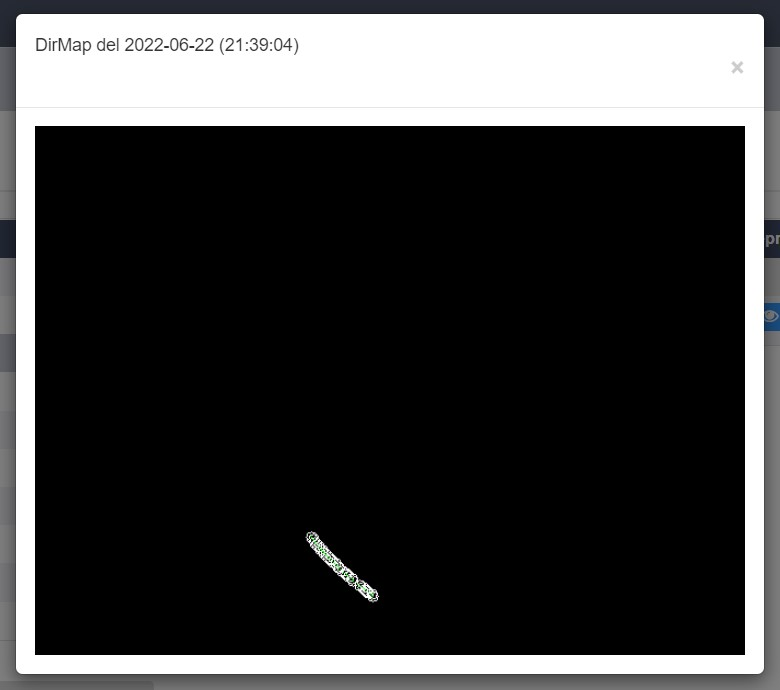
\includegraphics[width=0.85\textwidth]{images/dirmap.jpg}
        \end{center}
    \end{subfigure}
    \begin{subfigure}{\textwidth}
        \begin{center}
        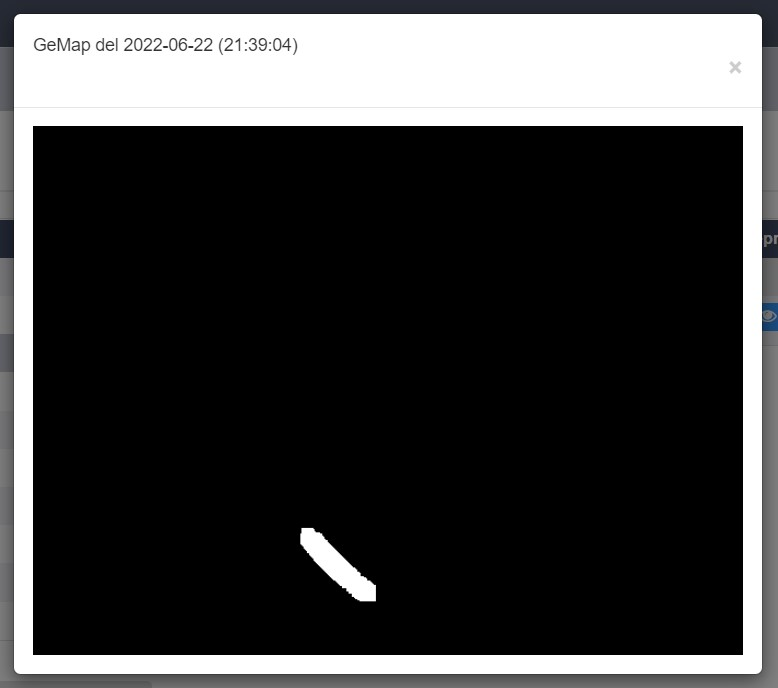
\includegraphics[width=0.85\textwidth]{images/gemap.jpg}
        \end{center}
    \end{subfigure}
    \caption{DirMap e GeMap della detection del 22/06/2022.}
\end{figure}




\section{Homepage}
La web application dispone di una homepage che riporta i dati più significativi inerenti alla stazione.

\begin{figure}[H]
    \begin{center}
    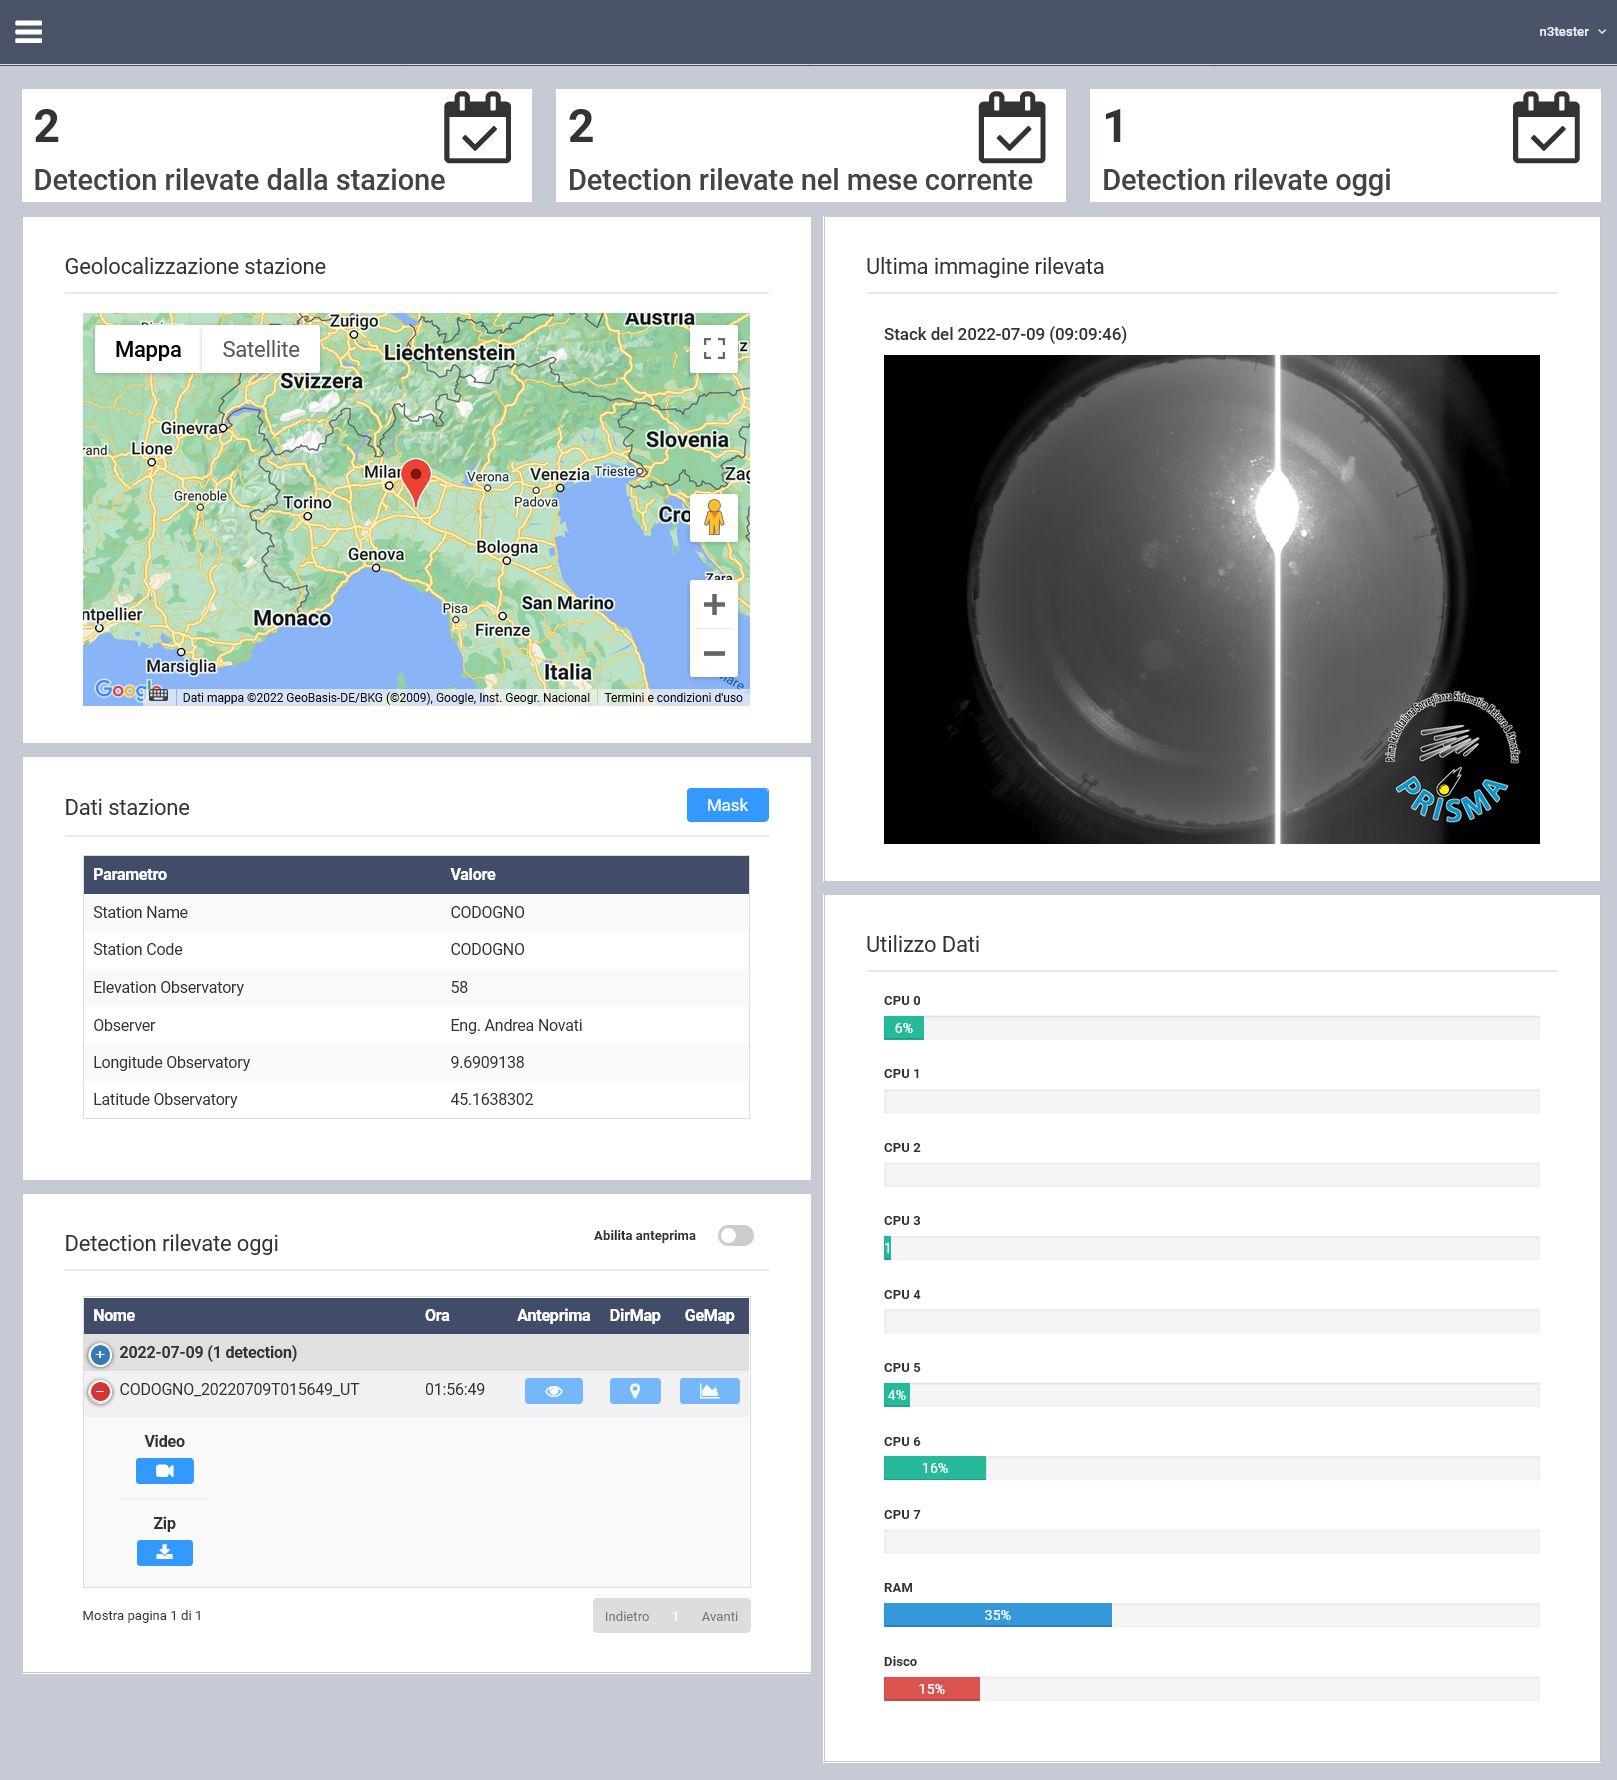
\includegraphics[width=\textwidth]{images/full-home.png}
    \caption{\emph{Homepage} della web application.}
    \label{fig:homepage}
    \end{center}
\end{figure}

\subsection{Visualizzazione metriche}

All'inizio della pagina sono indicati alcuni dati numerici relativi alle detection rilevate:
\begin{itemize}[noitemsep,nolistsep]
    \item Numero di detection rilevate dalla stazione \textbf{totali}
    \item Numero di detection rilevate dalla stazione \textbf{nel mese corrente}
    \item Numero di detection rilevate dalla stazione \textbf{oggi}
\end{itemize}

\begin{figure}[H]
    \begin{center}
    
\includegraphics[width=\textwidth]{images/metriche.png}
    \caption{Metriche.}
    \end{center}
\end{figure}

\subsection{Geolocalizzazione e informazioni della stazione}

L'utente può visualizzare le \textbf{informazioni principali} della stazione (cfr. sezione \ref{ft-conf-automatica}) in una tabella; la \textbf{geolocalizzazione}, realizzata con GoogleMaps, (cfr. figura \ref{fig:homepage}) ed infine, se presente, la \textbf{maschera}, mostrata in una finestra modale, con possibilità di download.

\begin{figure}[H]
    \begin{center}
    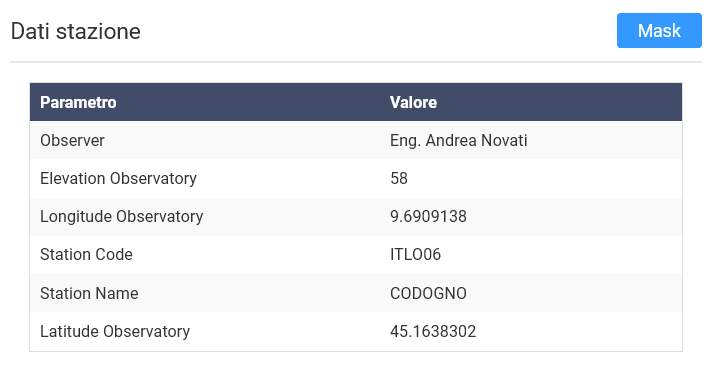
\includegraphics[width=\textwidth]{images/dati-stazione.png}
    \caption{Dati princiapli della stazione.}
    \end{center}
\end{figure}
\begin{figure}[H]
    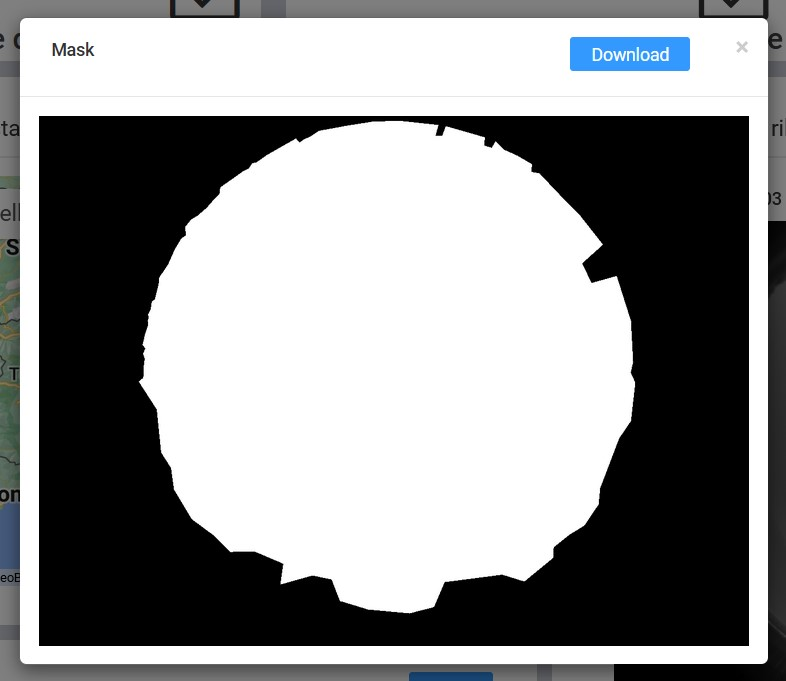
\includegraphics[width=\textwidth]{images/mask.jpg}
    \caption{Anteprima della maschera.}
\end{figure}

\subsection{Visualizzazione ultime detection}

Sotto i dati della stazione, si possono consultare le detection rilevate nell'ultimo giorno. La tabella in questione coincide con la seconda tabella nella sezione \emph{Detection}, associata all'ultima data disponibile (cfr. sezione \ref{detec-tables}).

Viene inoltre riportata nella homepage l'immagine dell'\textbf{ultimo stack}, che coincide con l'ultima immagine rilevata dalla stazione.

\subsection{Visualizzazione stato risorse dell'hardware} \label{stato-risorse-hw}

L'utente visionando la homepage può avere una panoramica dell'\textbf{utilizzo delle risorse} sul nodo (cfr. figura \ref{fig:homepage}). Sono infatti riportati:
\begin{itemize}[noitemsep,nolistsep]
    \item Utilizzo \textbf{CPU} (è riportato l'utilizzo di ciascun core)
    \item Utilizzo \textbf{RAM}
    \item Occupazione \textbf{disco}
\end{itemize}

Il client effettua una richiesta al server ogni 5 secondi per aggiornare i dati. 

Il server per trovare l'utilizzo di ciascun core tramite il software sysstat (cfr. sezione \ref{software}) esegue il comando \texttt{mpstat}, ricavando i dati necessari con \texttt{awk} (cfr. listing \ref{lst:system-usage}).

\begin{lstlisting}[style=PHP,caption={Metodo PHP per ottenere l'utilizzo di CPU, RAM e disco.},captionpos=b,label={lst:system-usage}]
    // Get percentage values of cpu, ram and disk usage
    public static function getStoragePercentage() {
        $disk = ((disk_total_space("/") 
            - disk_free_space("/"))
            / disk_total_space("/")) * 100;
        $cpu = array();
        $i = 0;
        while (true) {
            $core = shell_exec("mpstat -P $i 1 1 | awk
                'FNR==4
                {print($3+$4+$5+$6+$7+$8+$9+$10+$11)}'");
            if (is_null($core)) {
                break;
            }
            $cpu[] = (float) str_replace("\n", "", $core);
            $i++;
        }
        $free1 = shell_exec('free');
        $free2 = (string) trim($free1);
        $free_arr = explode("\n", $free2);
        $mem1 = explode(" ", $free_arr[1]);
        $mem2 = array_filter($mem1);
        $mem3 = array_merge($mem2);
        $ram = $mem3[2] / $mem3[1] * 100;
        return array($cpu, $ram, $disk);
    }
\end{lstlisting}

\section{Impostazioni}
In alto a destra sulla toolbar è presente un \textbf{menu a tendina}, che permette all'utente due operazioni:
\begin{enumerate}[noitemsep,nolistsep]
    \item Effettuare il \textbf{logout};
    \item Accedere alle \textbf{impostazioni} (solo per utenti di livello \emph{Admin}).
\end{enumerate}
\begin{figure}[H]
    
\includegraphics[width=\textwidth]{images/drop-down-menu.jpg}
    \caption{Menu a tendina per utenti di livello \emph{Admin}.}
\end{figure}
Nella pagina delle impostazioni (cfr. figura \ref{fig:settings}) sono presenti due sottosezioni principali:
\begin{itemize}[noitemsep,nolistsep]
    \item \emph{Visualizzazione Media}, per abilitare o disabilitare la visualizzazione delle anteprime o la creazione di video e archivi;
    \item \emph{Archiviazione Media}, per gestire lo spazio sul nodo.
\end{itemize}

\subsection{Disabilitazione visualizzazione anteprime}

Gli amministratori possono decidere, disattivando il \emph{toggle button} corrispondente, di non permettere a qualunque utente acceda alla web application del nodo in questione di visualizzare le anteprime delle sezioni \emph{Capture}, \emph{Stack} e \emph{Detection}, nel caso non si voglia appesantire il nodo con ulteriori elaborazioni ad esempio durante la notte.

\begin{figure}[H]
    
\includegraphics[width=\textwidth]{images/no-preview-toggle.jpg}
\end{figure}

\begin{figure}[H]
    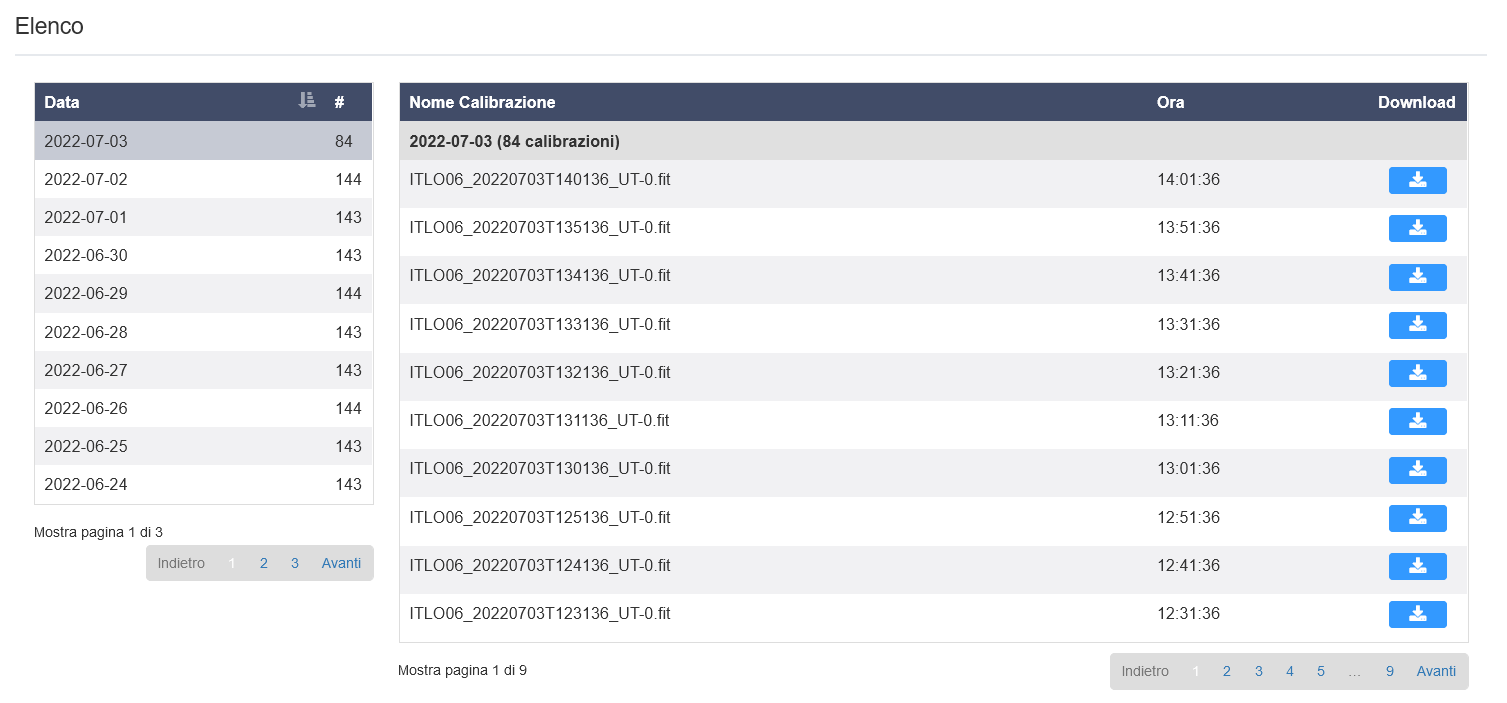
\includegraphics[width=\textwidth]{images/capture-no-preview.png}
    \caption{Sezione \emph{Capture} senza le anteprime. Si noti che non è più presente\emph{toggle button} per attivarle.}
\end{figure}

\subsection{Disabilitazione creazione video e archivio}

Disattivando invece il \emph{toggle button} riguardante i video e gli archivi, gli amministratori possono impedire a qualunque utente che acceda di richiedere lo scaricamento di video o di zip nella sezione \emph{Detection}. Il fine di questa scelta concerne sempre l'utilizzo della risorse sul nodo, soprattutto per non interferire con le elaborazioni del software FreeTure.

\begin{figure}[H]
    
\includegraphics[width=\textwidth]{images/no-download-toggle.jpg}
\end{figure}

\begin{figure}[H]
    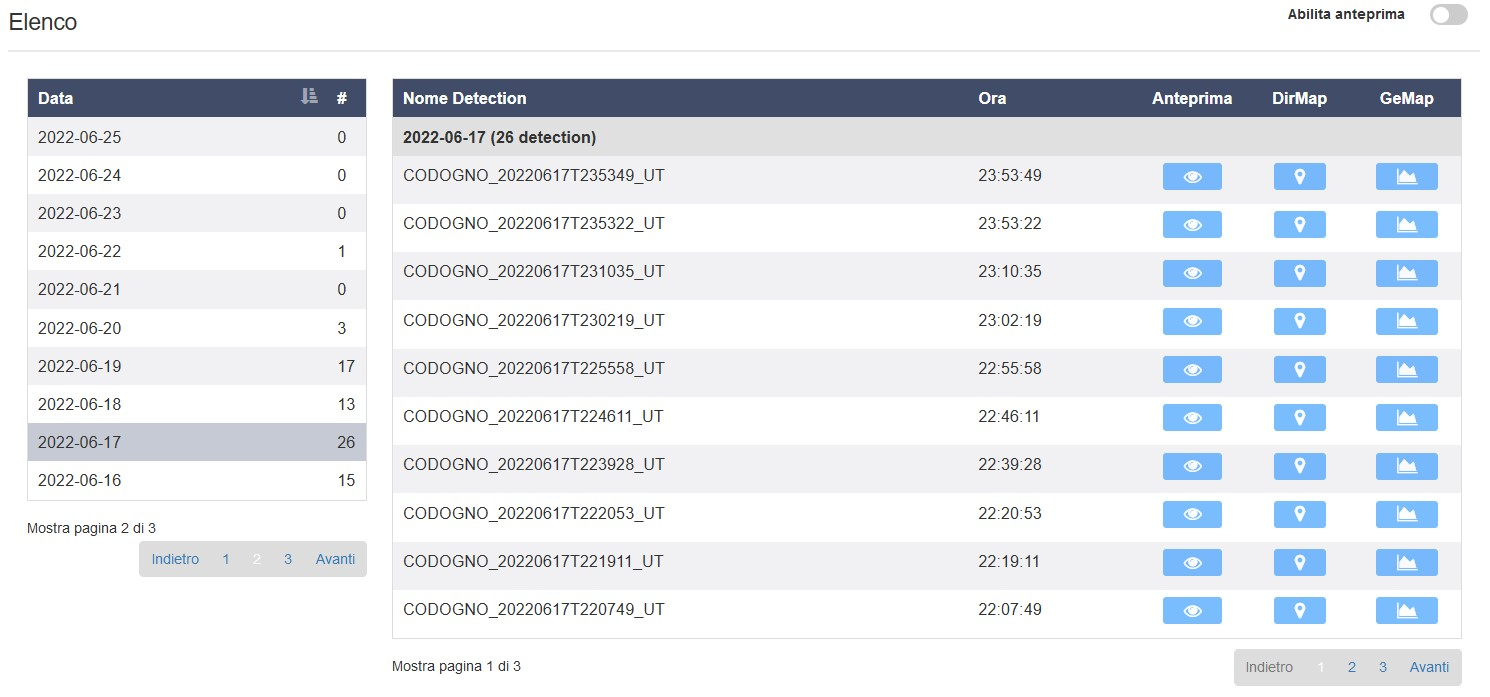
\includegraphics[width=\textwidth]{images/detection-no-download.jpg}
    \caption{Sezione \emph{Detection} senza possibilità di scaricare i video o gli archivi.}
\end{figure}

\subsection{Pulizia media provvisori} \label{clean-media}

\begin{wrapfigure}{r}{0.3\textwidth}
    \vspace{-10pt}
    
\includegraphics[width=0.3\textwidth]{images/clean-media-button.jpg}
    \vspace{-24pt}
\end{wrapfigure}
Nella sezione \ref{elaborazione-dati-detec} si era accennato al fatto che la gestione dei media provvisori sul disco era responsabilità dell'utente.
Nelle impostazioni un amministratore può \textbf{visualizzare quanto spazio occupano in memoria} i video e gli archivi creati precedentemente e quindi decidere se \textbf{liberare lo spazio}, cancellando i media.  

\begin{figure}[H]
    \begin{center}
    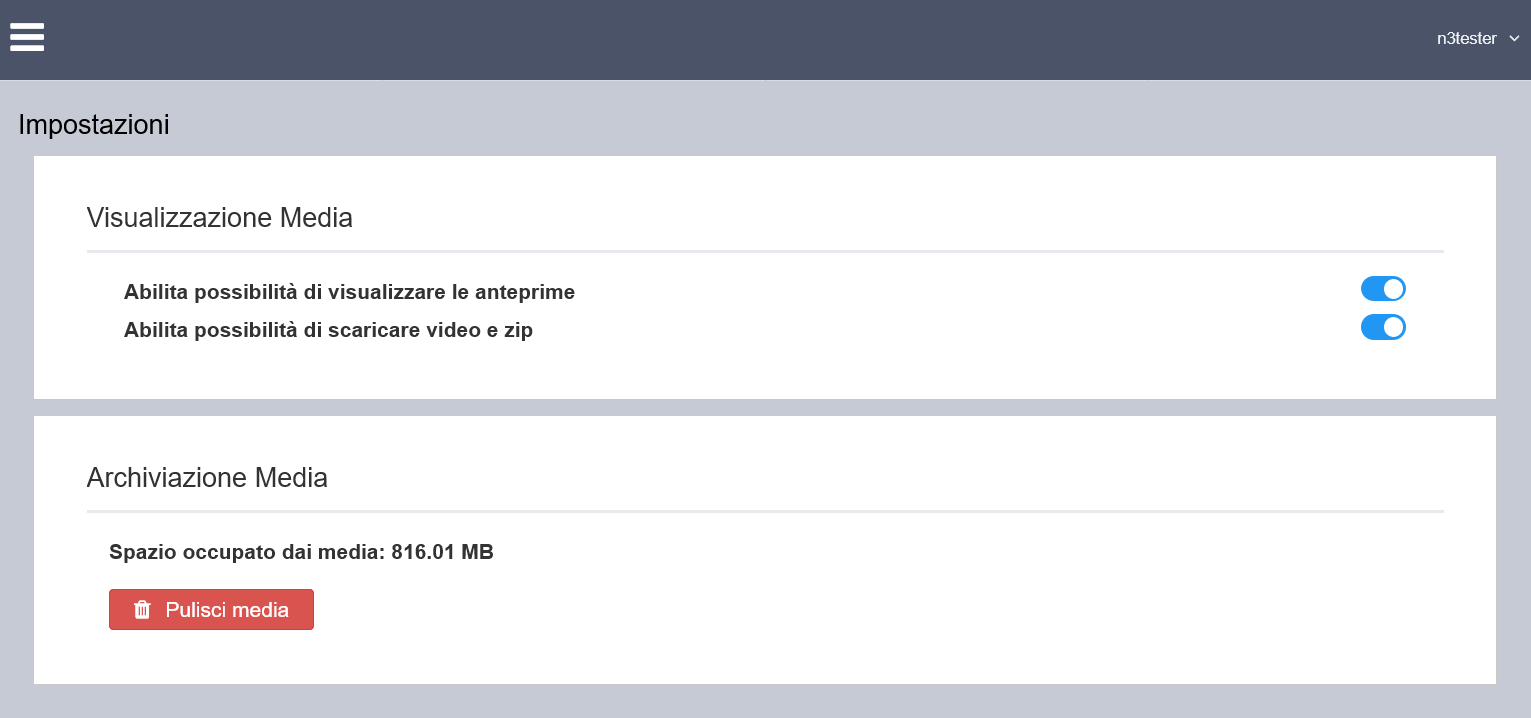
\includegraphics[width=\textwidth]{images/full-settings.png}
    \caption{\emph{Impostazioni}.}
    \label{fig:settings}
    \end{center}
\end{figure}

\chapter{Conclusioni}
\section{Sviluppi Futuri}
\subsection{Dashboard}

La web application oggetto del tirocinio è inerente solamente ai singoli nodi per la loro configurazione e per la consultazione dei dati raccolti. Pertanto, si è pianificato di implementare nel futuro una \emph{dashboard} operativa relativa al server di elaborazione centrale, che raccolga i dati da tutti i nodi e possa permettere all'utente una panoramica generale di tutta la rete PRISMA, per consultare anche gli eventi veri e propri generati dall'elaborazione delle detection.

\subsection{Realtà aumentata}

L'elaborazione dei dati raccolti dalle telecamere della rete, attraverso l'analisi delle immagini e il calcolo delle traiettorie e della magnitudine, genera dei file che riproducono tridimensionalmente l'evento (cfr. figura \ref{fig:bolide-050322}). A fronte di questo, l'INAF ha proposto di creare alcune esperienze in realtà aumentata per gli appassionati o per i più piccoli che riproducano in 3D la caduta della meteora.

\begin{figure}
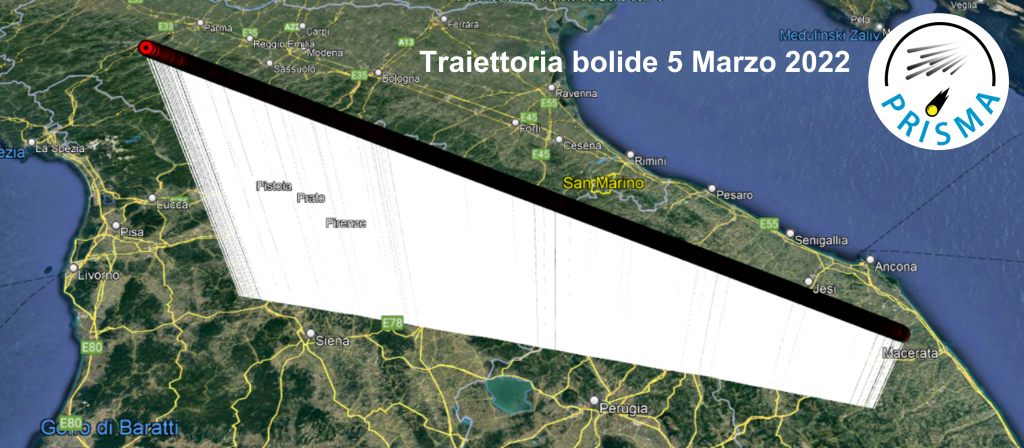
\includegraphics[width=\textwidth]{images/traiettoria-20220305.png}
\caption{Traiettoria del bolide del 5 marzo 2022. \cite{bolide-050322}}
\label{fig:bolide-050322}
\end{figure}

\subsection{Cloud computing}

Attualmente la rete PRISMA si appoggia per l'elaborazione ad un server centrale. Per il futuro si ha intenzione di spostare parte dell'analisi dei dati sui nodi della rete, in modo da non sovraccaricare un unico server e sfruttare la potenza computazionale di ciascuna delle macchine che compongono la rete. In particolar modo, si è pensato di far elaborare i dati dai nodi nelle ore diurne, quando il software FreeTure non è attivo.

\subsection{Integrazione con modelli AI}

Ad oggi, PRISMA basa tutte le sue elaborazioni dai dati raccolti mediante il software open-source FreeTure. È però in corso, sempre in collaborazione con l'azienda N3 Srl, una ricerca sull'implementazione di modelli di intelligenza artificiale più precisi ed efficienti rispetto a FreeTure. 

\section{Stato Attuale}
La web application che è stata illustrata in questa tesi è funzionante e operativa (si può consultare il codice su GitHub \cite{prisma-node-webmin}). Durante il tirocinio sono stati configurati due nodi in produzione, Codogno e Savelli, attualmente in funzione: il nodo di Codogno ha infatti rilevato il 22 giugno 2022 una meteora, ben visibile nella figura \ref{fig:codogno-2206} consultabile direttamente dalla web app.

La ricerca che si sta sviluppando attorno al progetto PRISMA è consistente e promettente, coinvolgendo numerosi appassionati e studenti da tutta Italia. Per mezzo di tutti questi contributi il progetto è funzionante e sta portando ottimi risultati: grazie ad esso oltre ad essere state individuate sono state già raccolte alcune meteore anche di piccole dimensioni, che altrimenti sarebbero passate inosservate.

\newpage
\addcontentsline{toc}{chapter}{Sitografia}
\printbibliography[title={Sitografia}]

\end{document}


